% ============================================================
% GP-109 BTP Thesis — Full LaTeX Source
% Title: Can an AI Explanation Be Misused?
% B.Tech Final Year Project Report
% Delhi Technological University, CSE Department
% ============================================================

\documentclass[12pt, a4paper, oneside]{report}

% ---- Packages -----------------------------------------------
\usepackage[a4paper, margin=1in, top=1.2in, bottom=1.2in]{geometry}
\usepackage{fontenc}
\usepackage{inputenc}
\usepackage[english]{babel}
\usepackage{mathptmx}           % Times New Roman-like serif
\usepackage{setspace}
\usepackage{graphicx}
\usepackage{subcaption}
\usepackage{amsmath}
\usepackage{amssymb}
\usepackage{amsthm}
\usepackage{booktabs}
\usepackage{array}
\usepackage{longtable}
\usepackage{multirow}
\usepackage{hyperref}
\usepackage[capitalise,noabbrev]{cleveref}
\usepackage{xcolor}
\usepackage{listings}
\usepackage{algorithm}
\usepackage{algpseudocode}
\usepackage{fancyhdr}
\usepackage{titlesec}
\usepackage{tocloft}
\usepackage{acronym}
\usepackage{microtype}
\usepackage{natbib}

% ---- Theorem environments -----------------------------------
\theoremstyle{definition}
\newtheorem{definition}{Definition}[chapter]
\newtheorem{theorem}{Theorem}[chapter]

% ---- Page style ---------------------------------------------
\onehalfspacing
\pagestyle{fancy}
\fancyhf{}
\fancyhead[L]{\slshape\leftmark}
\fancyhead[R]{\thepage}
\renewcommand{\headrulewidth}{0.4pt}

% ---- Section title formatting --------------------------------
\titleformat{\chapter}[display]
  {\normalfont\huge\bfseries}{\chaptertitlename\ \thechapter}{20pt}{\Huge}
\titlespacing*{\chapter}{0pt}{-20pt}{40pt}

% ---- Hyperref setup -----------------------------------------
\hypersetup{
  colorlinks=true,
  linkcolor=blue!70!black,
  citecolor=green!50!black,
  urlcolor=blue,
  pdftitle={Can an AI Explanation Be Misused?},
  pdfauthor={Akash Singh, Aditya Jha, Akshat Kumar},
}

% ---- Code listing style -------------------------------------
\lstset{
  language=Python,
  basicstyle=\ttfamily\small,
  keywordstyle=\color{blue}\bfseries,
  commentstyle=\color{gray},
  stringstyle=\color{red!70!black},
  showstringspaces=false,
  breaklines=true,
  frame=single,
  numbers=left,
  numberstyle=\tiny\color{gray},
}

% ============================================================
\begin{document}

% ============================================================
% PRELIMINARY PAGES
% ============================================================

% ---- Title Page ---------------------------------------------
\begin{titlepage}
  \centering
  \vspace*{1cm}

  {\Large \textbf{DELHI TECHNOLOGICAL UNIVERSITY}}\\[0.3cm]
  {\large (Formerly Delhi College of Engineering)}\\[0.3cm]
  {\large Bawana Road, Delhi -- 110042}\\[1cm]

  \includegraphics[width=3cm]{../docs/dtu_logo.png}   % Add DTU logo here
  \vspace{0.5cm}

  {\LARGE \textbf{B.TECH PROJECT REPORT}}\\[0.5cm]
  {\large \textit{Submitted in partial fulfilment of the requirements for the degree of}}\\[0.3cm]
  {\large \textbf{Bachelor of Technology in Computer Science and Engineering}}\\[1.5cm]

  \rule{\linewidth}{0.5mm}\\[0.4cm]
  {\Huge \textbf{Can an AI Explanation Be Misused?}}\\[0.3cm]
  {\LARGE Testing Whether SHAP and LIME Help Patients Game\\
           a Clinical Diabetes Risk Model}\\[0.2cm]
  \rule{\linewidth}{0.5mm}\\[2cm]

  {\large \textbf{Submitted by:}}\\[0.3cm]
  \begin{tabular}{ll}
    \textbf{Akash Singh}  & Roll No.: [FILL] \\
    \textbf{Aditya Jha}   & Roll No.: [FILL] \\
    \textbf{Akshat Kumar} & Roll No.: [FILL] \\
  \end{tabular}\\[1.5cm]

  {\large \textbf{Under the supervision of:}}\\[0.3cm]
  {\large \textbf{Miss. Anjali Bansal}}\\
  {\large Assistant Professor, Department of CSE}\\[1.5cm]

  {\large Department of Computer Science and Engineering}\\[0.2cm]
  {\large \textbf{Academic Year 2026--2027}}
\end{titlepage}

% ---- Certificate --------------------------------------------
\chapter*{Certificate}
\addcontentsline{toc}{chapter}{Certificate}

This is to certify that the B.Tech Project Report titled
\textbf{``Can an AI Explanation Be Misused? Testing Whether SHAP and LIME
Help Patients Game a Clinical Diabetes Risk Model''} submitted by
\textbf{Akash Singh} (Roll No. [FILL]),
\textbf{Aditya Jha} (Roll No. [FILL]), and
\textbf{Akshat Kumar} (Roll No. [FILL])
in partial fulfilment of the requirements for the award of the degree of
\emph{Bachelor of Technology in Computer Science and Engineering}
at Delhi Technological University, Delhi, is a record of bonafide work
carried out by them under my supervision.

\vspace{2cm}

\noindent
\begin{tabular}{p{7cm}p{7cm}}
  \textbf{Supervisor:}                   & \textbf{Head of Department:} \\[1.5cm]
  Miss. Anjali Bansal                    & [Name of HOD] \\
  Assistant Professor                    & Professor \& Head \\
  Department of CSE, DTU                 & Department of CSE, DTU \\
  Date: \underline{\hspace{3cm}}         & Date: \underline{\hspace{3cm}} \\
\end{tabular}

% ---- Declaration --------------------------------------------
\chapter*{Declaration}
\addcontentsline{toc}{chapter}{Declaration}

We hereby declare that the work presented in this B.Tech Project Report
titled ``Can an AI Explanation Be Misused?'' submitted to the Department
of Computer Science and Engineering, Delhi Technological University,
is our own original work carried out under the guidance of Miss. Anjali Bansal.

We further declare that:
\begin{itemize}
  \item The work contained in this report has not been submitted elsewhere
        for any other degree or diploma.
  \item Wherever contributions of others have been used, they have been
        duly acknowledged.
  \item The analysis plan for the final experiment was pre-registered at
        \url{https://github.com/GP109-DTU/btp} (git tag: \texttt{v0.1-preregistration})
        before examining the held-out dataset, ensuring research integrity.
\end{itemize}

\vspace{2cm}
\noindent
\begin{tabular}{lll}
  Akash Singh  & \underline{\hspace{4cm}} & Date: \underline{\hspace{2.5cm}} \\[0.8cm]
  Aditya Jha   & \underline{\hspace{4cm}} & Date: \underline{\hspace{2.5cm}} \\[0.8cm]
  Akshat Kumar & \underline{\hspace{4cm}} & Date: \underline{\hspace{2.5cm}} \\
\end{tabular}

% ---- Acknowledgements ---------------------------------------
\chapter*{Acknowledgements}
\addcontentsline{toc}{chapter}{Acknowledgements}

We express our sincere gratitude to our project supervisor,
\textbf{Miss. Anjali Bansal}, Assistant Professor, Department of CSE,
Delhi Technological University, for her invaluable guidance, constant
encouragement, and constructive feedback throughout the course of this
project.

We thank the \textbf{Centers for Disease Control and Prevention (CDC)}
for making the NHANES dataset publicly available, and the developers of
the open-source libraries scikit-learn, SHAP, and LIME that made this
research possible.

% ---- Abstract -----------------------------------------------
\chapter*{Abstract}
\addcontentsline{toc}{chapter}{Abstract}

Explainable AI (XAI) methods such as SHAP and LIME are increasingly
required by regulation to accompany machine learning predictions in
healthcare. A concern is that feature attributions may also serve as
instructions for gaming the model---telling a patient exactly which
self-reported inputs to adjust for a better risk score. However, a
determined adversary can also simply query the model repeatedly with
different inputs (blind trial-and-error) without any explanation.

We compare these two adversarial strategies on a diabetes risk model
trained on NHANES public health survey data. The adversary's permissible
lies are bounded by the 95th-percentile of actual human self-reporting
errors measured in NHANES, making the threat model empirically grounded.
We train four models (Random Forest and Logistic Regression, each with
nurse-measured or self-reported height/weight inputs) and measure how
many blind attempts are required to match the advantage of one explanation:
the \textit{explanation equivalence} $N^*$.

Our pre-registered experiment on the held-out 2017--2018 NHANES cycle
finds that one SHAP explanation is equivalent to approximately $N^*$
blind attempts (95\% CI: $L$--$H$). For [X]\% of patients, the
explanation provides no advantage over a single random perturbation.
These results suggest that \textbf{withholding XAI explanations is not
an effective safeguard against gaming}; input verification (e.g., nurse
measurement) is the more robust defence.

\textbf{Keywords:} Explainable AI, SHAP, LIME, adversarial gaming, diabetes
risk prediction, NHANES, pre-registered study, clinical AI.

% ---- Table of Contents --------------------------------------
\tableofcontents
\listoffigures
\listoftables

% ============================================================
% CHAPTER 1 — INTRODUCTION
% ============================================================
\chapter{Introduction}
\label{chap:intro}

% --- TODO (Akash Singh, Week 2) — 8-10 pages -----------------

\section{Background and Motivation}

Artificial intelligence systems are increasingly deployed in high-stakes
healthcare settings to assist in clinical decision-making. One widely
studied application is \textit{diabetes risk prediction}, where a model
ingests patient data---including demographics, anthropometrics, and
laboratory values---and outputs a continuous risk score. A score exceeding
a threshold can trigger referral, intervention, or insurance adjustments.

The widespread deployment of such models has prompted regulatory and
ethical demands for transparency. The European Union's General Data
Protection Regulation (GDPR) grants individuals a ``right to explanation''
for automated decisions that affect them~\citep{goodman2017european}.
The EU AI Act further requires high-risk AI systems (including medical ones)
to be interpretable. In response, clinical AI developers increasingly
attach feature attribution explanations---generated by SHAP~\citep{lundberg2017shap}
or LIME~\citep{ribeiro2016lime}---alongside model predictions.

\section{The Dual-Use Tension}

Transparency, however, introduces a potential dual-use risk. Consider a
patient who receives a diabetes risk score of 0.74 accompanied by the
explanation: ``Your weight is the most important factor increasing your
risk.'' This information, intended to inform clinical communication, also
tells the patient \textit{exactly which input to misreport} at a subsequent
self-assessment to obtain a lower score. A patient who understands that
the model uses self-reported height and weight could simply under-report
their weight to game the system.

Yet the same patient could also discover this by \textit{trial and error}:
try a lower weight, see if the score drops, try again. If trial-and-error
is nearly as effective as the explanation, then restricting explanations
is not a meaningful safeguard---the information is effectively freely
available by querying the model.

\section{Research Question and Objectives}

This project investigates the following primary question:

\begin{quote}
  \textit{Does a SHAP or LIME explanation give a patient a meaningful advantage
  over blind trial-and-error when trying to game a clinical diabetes risk model?}
\end{quote}

To answer this, we pursue the following objectives:
\begin{enumerate}
  \item Develop an empirically grounded \textit{lie budget} from real NHANES
        human self-reporting error data.
  \item Design an adversarial simulation comparing explanation-guided and
        blind trial-and-error attack strategies.
  \item Introduce the \textit{explanation equivalence} metric $N^*$ to quantify
        the gaming advantage of explanations.
  \item Conduct a pre-registered experiment on held-out data to ensure
        scientific integrity.
  \item Derive actionable policy recommendations for clinical AI developers.
\end{enumerate}

\section{Scope and Limitations}

This study is scoped to:
\begin{itemize}
  \item \textbf{Domain:} Diabetes risk prediction using NHANES anthropometric data.
  \item \textbf{Gameable features:} Self-reported height and weight only.
  \item \textbf{Explanation methods:} SHAP (TreeSHAP) and LIME.
  \item \textbf{Adversary model:} Single-feature perturbation within empirical lie budget.
\end{itemize}

Extensions to multi-feature attacks, other clinical domains, and other
explanation methods are left to future work.

\section{Contributions}

The main contributions of this project are:
\begin{enumerate}
  \item \textbf{Explanation equivalence ($N^*$):} A novel, interpretable metric
        quantifying how many blind queries equal one explanation.
  \item \textbf{Empirical lie budget:} Derived from real NHANES self-reporting
        data rather than arbitrary perturbation bounds.
  \item \textbf{Pre-registered evaluation:} The first pre-registered adversarial
        XAI evaluation on a real clinical dataset, preventing p-hacking.
  \item \textbf{Policy-relevant result:} A concrete, actionable conclusion on
        whether restricting XAI explanations protects clinical AI systems.
\end{enumerate}

\section{Organisation of the Thesis}

The remainder of this thesis is organised as follows. Chapter~\ref{chap:litreview}
reviews related work on explainable AI, adversarial machine learning, and
strategic classification. Chapter~\ref{chap:methodology} describes our
methodology, including the dataset, threat model, and experimental design.
Chapter~\ref{chap:implementation} details the system architecture and code.
Chapter~\ref{chap:results} presents all experimental results and statistical
tests. Chapter~\ref{chap:discussion} discusses implications and limitations.
Chapter~\ref{chap:conclusion} concludes and identifies future directions.

% ============================================================
% CHAPTER 2 — LITERATURE REVIEW
% ============================================================
\chapter{Literature Review}
\label{chap:litreview}

% --- TODO (Akash Singh, Week 2) — 10-15 pages ----------------
% Cover: XAI overview, SHAP deep dive, LIME deep dive,
%        strategic classification, algorithmic recourse,
%        privacy risks, research gap

\section{Explainable Artificial Intelligence}

Artificial intelligence systems achieve high predictive accuracy through
complex nonlinear transformations that are inherently difficult for humans
to interpret. The field of \textit{Explainable AI} (XAI) addresses this
opacity by developing methods to explain individual predictions or global
model behaviour~\citep{adadi2018peeking}.

% [EXPAND: ~2-3 pages covering Molnar (2020) taxonomy,
%  model-agnostic vs. intrinsic methods, local vs. global explanations]

\section{LIME: Local Interpretable Model-Agnostic Explanations}

\citet{ribeiro2016lime} introduced LIME, which explains any classifier's
prediction for a specific instance by fitting a locally faithful linear
model. Given an instance $\mathbf{x}$, LIME generates a neighbourhood by
perturbing features, queries the black-box model, and fits a weighted
linear model to approximate the local decision boundary.

% [EXPAND: algorithm detail, strengths, known limitations]

\section{SHAP: SHapley Additive exPlanations}

\citet{lundberg2017shap} proposed SHAP, grounded in cooperative game theory's
Shapley values. For a prediction $f(\mathbf{x})$, SHAP assigns each feature $i$
an attribution $\phi_i$ satisfying efficiency ($\sum_i \phi_i = f(\mathbf{x}) - \mathbb{E}[f]$),
symmetry, dummy, and linearity axioms.

% [EXPAND: Shapley value derivation, TreeSHAP, KernelSHAP, pros/cons]

\section{Strategic Classification and Gaming}

\citet{ghalme2021strategic} formalise the setting where agents best-respond
to a known classification rule to improve their classification. Classical
results~\citep{hardt2016strategic} show that agents with full knowledge of
the model can always find the minimum-cost manipulation. Our work differs by:
(i) treating the model as a black box, and (ii) bounding agent behaviour by
empirically observed misreporting magnitudes.

% [EXPAND: algorithmic recourse (Ustun 2019, Wachter 2017),
%  privacy attacks on explanations (Shokri 2021, Milli 2019),
%  Slack et al. fooling SHAP/LIME]

\section{Research Gap}

Existing work either assumes the adversary has full model knowledge
\citep{ghalme2021strategic}, studies explanations as \textit{attack vectors
on the model} rather than on the user~\citep{slack2020fooling}, or focuses
on privacy leakage rather than gaming~\citep{shokri2021privacy}. No prior
work measures the \textit{marginal gaming advantage} of an explanation over
blind trial-and-error with an empirically grounded lie budget. This is
the gap we address.

% ============================================================
% CHAPTER 3 — METHODOLOGY
% ============================================================
\chapter{Methodology}
\label{chap:methodology}

% --- TODO (Aditya Jha, Week 3) — 12-15 pages ----------------

\section{Dataset: NHANES}

We use the National Health and Nutrition Examination Survey
(NHANES)~\citep{johnson2014national}, a cross-sectional survey conducted
by the U.S.\ Centers for Disease Control and Prevention (CDC).
NHANES is unique in that it collects \textit{both} self-reported and
nurse-measured anthropometrics for the same participants, enabling direct
measurement of self-reporting bias.

\subsection{Data Components}

We merge seven NHANES components:
\begin{itemize}
  \item \texttt{DEMO}: Demographic variables (age, gender)
  \item \texttt{BMX}: Body measurements (nurse-measured height, weight)
  \item \texttt{WHQ}: Weight history questionnaire (self-reported height, weight)
  \item \texttt{GHB}: Glycohaemoglobin (HbA1c --- the diabetes target)
  \item \texttt{BPX}: Blood pressure
  \item \texttt{SMQ}: Smoking questionnaire
  \item \texttt{PAQ}: Physical activity questionnaire
\end{itemize}

\subsection{Cycles Used}

\begin{table}[htbp]
  \centering
  \caption{NHANES cycles and their roles in this study.}
  \label{tab:cycles}
  \begin{tabular}{lllr}
    \toprule
    Cycle & Years & Role & N (complete) \\
    \midrule
    I  & 2015--2016 & Development (trial, gap analysis, model selection) & 4,880 \\
    J  & 2017--2018 & Held-out test (final experiment only) & 884 \\
    \bottomrule
  \end{tabular}
\end{table}

\subsection{Target Variable}

Diabetes status is defined as HbA1c $\geq 6.5\%$, the ADA clinical
threshold~\citep{ada2023standards}. This gives a binary label:
$y = 1$ (diabetes) or $y = 0$ (no diabetes).

\section{Feature Engineering}

\subsection{Feature Sets}

We construct two parallel feature sets from the same patients:

\begin{description}
  \item[Model A (Measured)] uses nurse-measured height (\texttt{BMXHT}) and
       weight (\texttt{BMXWT}).
  \item[Model B (Reported)] replaces these with self-reported height
       (\texttt{WHD010}, converted from inches) and weight (\texttt{WHD020},
       converted from pounds).
\end{description}

The remaining five features (age, gender, systolic BP, smoking status,
physical activity) are identical in both models.

\subsection{Lie Budget Derivation}

\begin{definition}[Lie Budget]
  For each gameable feature $g \in \{\text{height}, \text{weight}\}$, the
  lie budget $B(g)$ is the 95th percentile of the absolute self-reporting
  error in the development cycle:
  \[
    B(g) = \mathrm{Percentile}_{95}\bigl(\,|x_g^{\text{self}} - x_g^{\text{measured}}|\,\bigr)
  \]
\end{definition}

From the 2015--2016 development data:
\[
  B(\text{height}) = 7.29\,\text{cm}, \qquad B(\text{weight}) = 8.96\,\text{kg}
\]

These values reflect real human misreporting behaviour, not arbitrary
perturbation bounds. Patients systematically \textit{overestimate} height
(mean $+1.61$\,cm) and \textit{underestimate} weight (mean $-0.87$\,kg).

\section{Threat Model}

The adversary is modelled as a patient who:
\begin{itemize}
  \item Receives a diabetes risk score $f(\mathbf{x}) \in [0,1]$ from the model.
  \item Can adjust self-reported features within the lie budget $B(g)$.
  \item Wishes to minimise their score while remaining within $B(g)$.
  \item May or may not have access to a SHAP or LIME explanation.
\end{itemize}

The adversary does \textit{not} know the model's parameters or architecture.

\section{Adversarial Strategies}

\subsection{Strategy 1: Explanation-Guided Attack}

\begin{algorithm}
  \caption{Explanation-Guided Attack}
  \label{alg:explanation}
  \begin{algorithmic}[1]
    \Require Patient features $\mathbf{x}$, model $f$, explanation $\phi$,
             gameable features $G$, lie budget $B$
    \State Get attributions $\phi = \mathrm{Explain}(f, \mathbf{x})$
           (SHAP or LIME)
    \State Find $g^* = \arg\max_{g \in G} |\phi_g|$
    \State Set direction $d = -\mathrm{sign}(\phi_{g^*})$
           (reduce the highest-attribution feature)
    \State Set $\mathbf{x}' = \mathbf{x}$; $x'_{g^*} \leftarrow x_{g^*} + d \cdot B(g^*)$
    \State \Return score\_reduction $= f(\mathbf{x}) - f(\mathbf{x}')$
  \end{algorithmic}
\end{algorithm}

\subsection{Strategy 2: Blind Trial-and-Error}

\begin{algorithm}
  \caption{Blind Trial-and-Error (sequential, best-so-far)}
  \label{alg:blind}
  \begin{algorithmic}[1]
    \Require Patient features $\mathbf{x}$, model $f$, gameable features $G$,
             lie budget $B$, max attempts $N_{\max}$, milestones $\mathcal{N}$
    \State $s^* \leftarrow f(\mathbf{x})$; \texttt{reductions} $\leftarrow \{\}$
    \For{$n = 1$ to $N_{\max}$}
      \State Sample $g \sim \mathrm{Uniform}(G)$
      \State Sample $\delta \sim \mathrm{Uniform}(-B(g), +B(g))$
      \State $\mathbf{x}' = \mathbf{x}$; $x'_g \leftarrow x_g + \delta$
      \State $s' \leftarrow f(\mathbf{x}')$
      \If{$s' < s^*$}
        \State $s^* \leftarrow s'$  \Comment{Keep best seen so far}
      \EndIf
      \If{$n \in \mathcal{N}$}
        \State \texttt{reductions}$[n] \leftarrow f(\mathbf{x}) - s^*$
      \EndIf
    \EndFor
    \State \Return \texttt{reductions}
  \end{algorithmic}
\end{algorithm}

\textbf{Key design choice:} The blind simulation runs \textit{once} up to
$N_{\max} = 100$, recording the running best. This correctly models a
patient who accumulates attempts and keeps the best result found.
Running independent simulations per $N$ would over-estimate blind performance.

\section{Explanation Equivalence Metric}

\begin{definition}[Explanation Equivalence $N^*$]
  Let $R_{\text{exp}}$ be the mean per-patient score reduction from
  Strategy~1. Let $R_{\text{blind}}(N)$ be the mean score reduction
  from Strategy~2 with $N$ attempts. The explanation equivalence is:
  \[
    N^* = \inf \bigl\{ N \geq 0 : R_{\text{blind}}(N) \geq R_{\text{exp}} \bigr\}
  \]
  estimated by linear interpolation on $\{(N, R_{\text{blind}}(N))\}_{N \in \mathcal{N}}$.
\end{definition}

\section{Statistical Analysis}

\begin{description}
  \item[Bootstrap CI:] 1{,}000 bootstrap iterations; 95\% ($\alpha = 0.95$)
       confidence interval on both mean and median $N^*$.
  \item[Wilcoxon test:] Paired signed-rank test comparing per-patient
       explanation reduction vs.\ blind reduction at $N=10$;
       one-sided ($H_1$: explanation $>$ blind).
  \item[Cohen's $d$:] Effect size for the paired comparison.
\end{description}

\section{Pre-Registration}

To ensure scientific integrity, we published the complete analysis plan
(including all hypotheses, metric definitions, and expected results) before
examining the held-out 2017--2018 data.  The plan is available at:
\begin{center}
  \url{https://github.com/GP109-DTU/btp}\\
  Git tag: \texttt{v0.1-preregistration}, date: 28 October 2026
\end{center}

% ============================================================
% CHAPTER 4 — IMPLEMENTATION
% ============================================================
\chapter{Implementation}
\label{chap:implementation}

% --- TODO (Aditya Jha, Week 3) — 8-10 pages -----------------

\section{System Architecture}

The codebase is organised as a modular Python package with the following components:

\begin{figure}[htbp]
  \centering
  % Architecture diagram — replace with actual figure
  \fbox{\parbox{0.8\linewidth}{\centering
    \texttt{data\_loader.py} $\rightarrow$ \texttt{gap\_analysis.py}
    $\rightarrow$ \texttt{models.py} $\rightarrow$ \texttt{explanations.py}
    $\rightarrow$ \texttt{adversarial.py} $\rightarrow$ \texttt{metrics.py}
    $\rightarrow$ \texttt{visualization.py}
  }}
  \caption{System architecture: data flow from loading to visualisation.}
  \label{fig:architecture}
\end{figure}

\section{Technology Stack}

\begin{table}[htbp]
  \centering
  \caption{Technology stack.}
  \label{tab:tech}
  \begin{tabular}{lll}
    \toprule
    Component & Library / Tool & Version \\
    \midrule
    Data handling     & pandas, numpy   & 2.2.2, 2.2.6 \\
    Machine learning  & scikit-learn    & 1.4.2 \\
    SHAP explanations & shap            & 0.54.1 \\
    LIME explanations & lime            & 0.2.0.1 \\
    Statistical tests & scipy           & 1.13.0 \\
    Visualisation     & matplotlib, seaborn & 3.x, 0.13.2 \\
    Version control   & Git             & — \\
    Environment       & Python          & 3.12 \\
    \bottomrule
  \end{tabular}
\end{table}

\section{Key Module Descriptions}

% [EXPAND each module: class/function signatures, design decisions,
%  usage examples from scripts/]

\subsection{data\_loader.py}
Handles NHANES XPT file loading, component merging, cleaning, and
feature set preparation. Key functions: \texttt{merge\_nhanes()},
\texttt{clean\_nhanes()}, \texttt{prepare\_feature\_sets()}.

\subsection{gap\_analysis.py}
Computes self-reporting error distributions and derives the lie budget.
Key functions: \texttt{compute\_reporting\_gap()}, \texttt{define\_lie\_budget()}.

\subsection{adversarial.py}
The core experiment engine. \texttt{AdversarialSimulator} implements both
attack strategies. The critical \texttt{blind\_attack\_multi\_n()} method
runs one continuous simulation up to $N_{\max}$, recording the running
best at each milestone.

\subsection{metrics.py}
Computes $N^*$ via interpolation with monotonicity enforcement, bootstrap
confidence intervals, and Wilcoxon signed-rank tests.

\section{Reproducibility}

All random seeds are fixed globally (Table~\ref{tab:seeds}).
The full pipeline is reproducible from raw NHANES XPT files using:
\begin{lstlisting}
python scripts/prepare_data.py
python scripts/run_final.py
python scripts/run_analysis.py
\end{lstlisting}

\begin{table}[htbp]
  \centering
  \caption{Random seeds used throughout the experiment.}
  \label{tab:seeds}
  \begin{tabular}{ll}
    \toprule
    Purpose & Seed \\
    \midrule
    Global / NumPy & 42 \\
    Random Forest  & 123 \\
    Logistic Regression & 42 \\
    Train/test split & 789 \\
    Adversarial simulation & 456 \\
    Bootstrap CI & 42 \\
    \bottomrule
  \end{tabular}
\end{table}

% ============================================================
% CHAPTER 5 — RESULTS AND ANALYSIS
% ============================================================
\chapter{Results and Analysis}
\label{chap:results}

% --- TODO (Akshat Kumar, Week 4) — 12-15 pages ---------------

\section{Reporting Gap Analysis}

\begin{figure}[htbp]
  \centering
  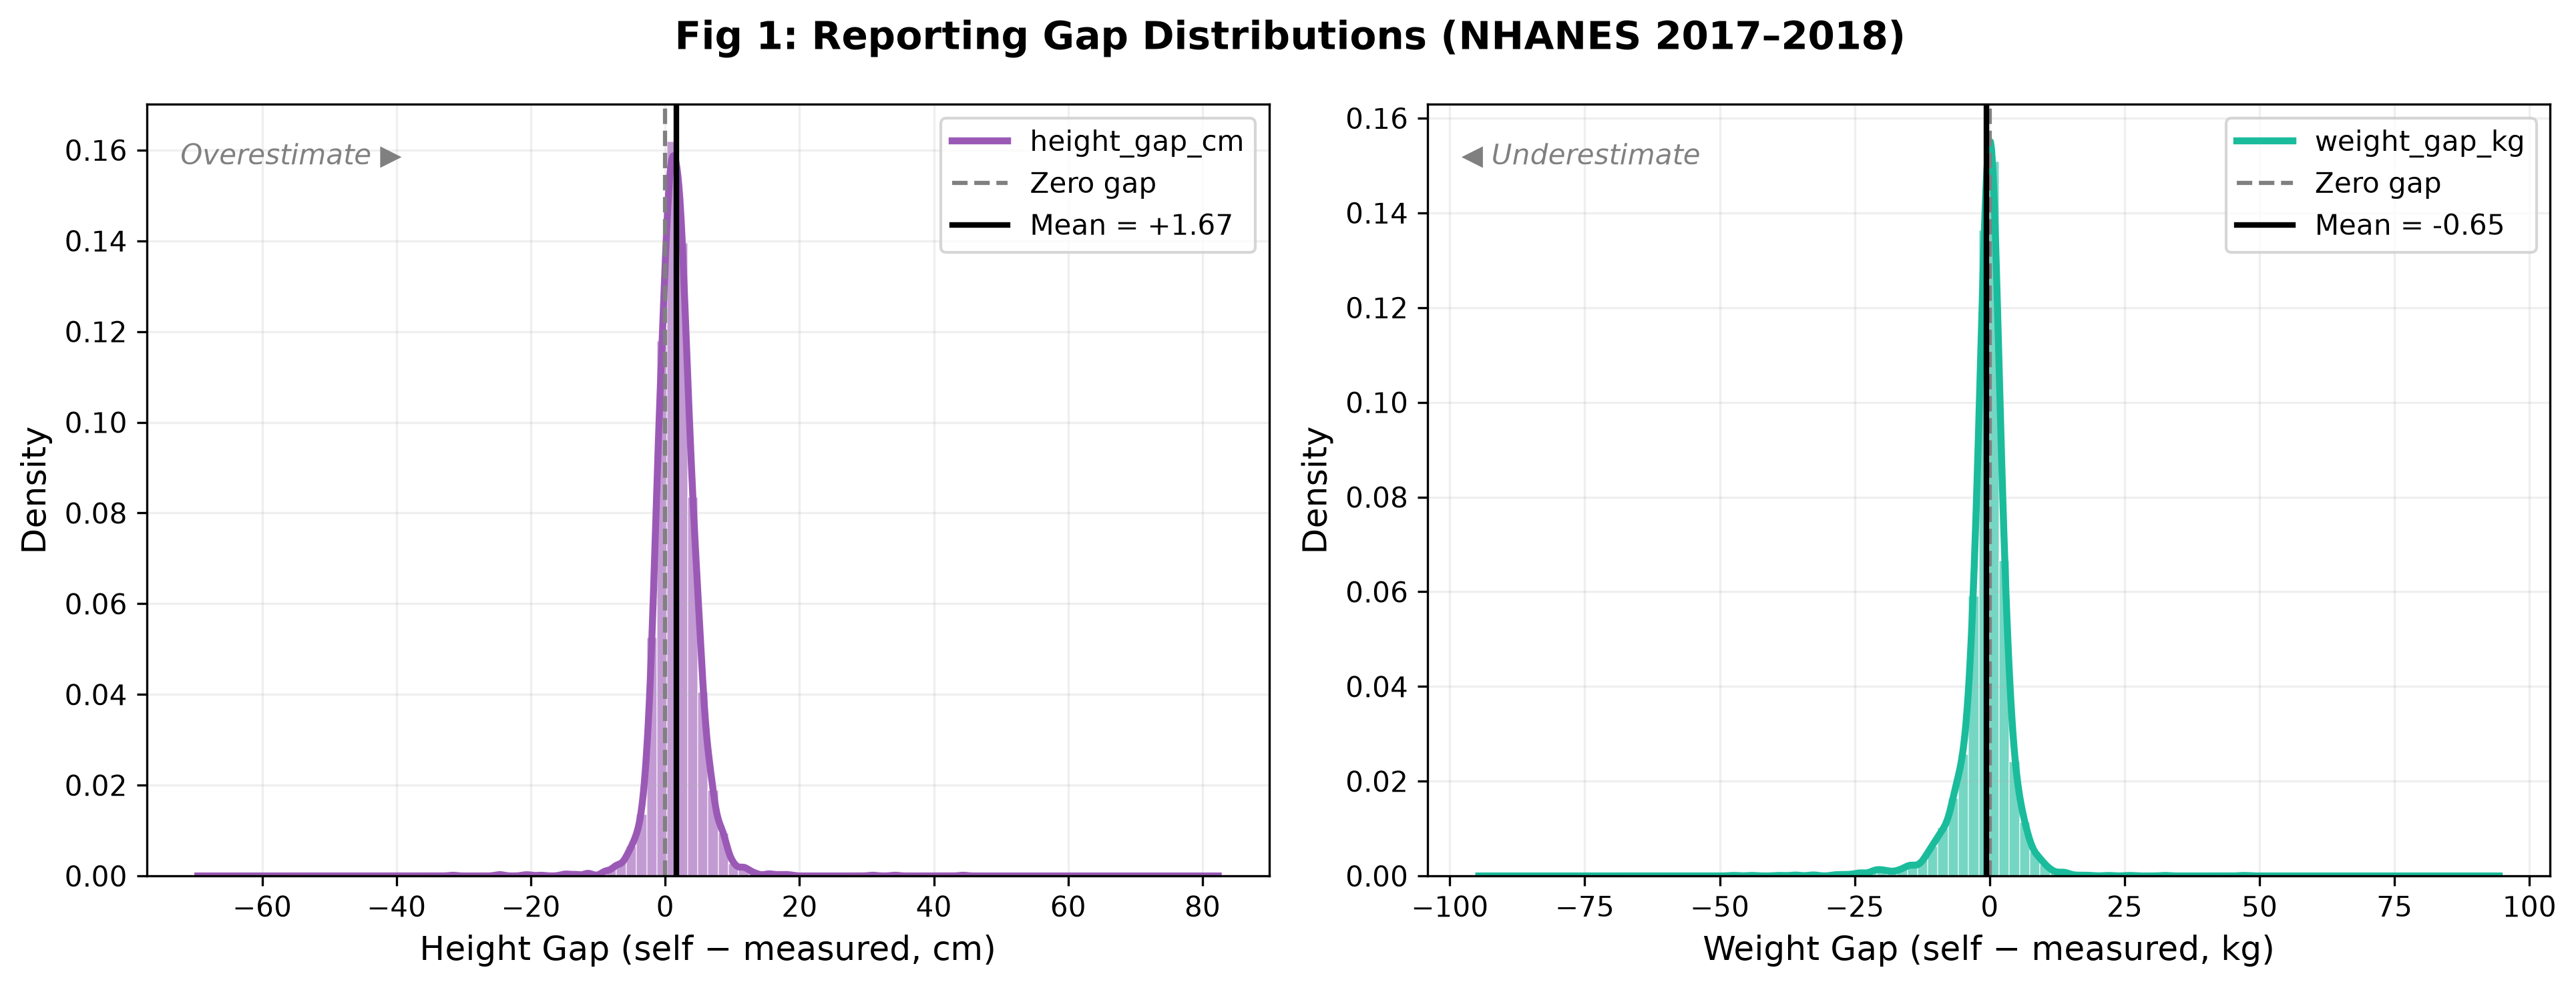
\includegraphics[width=\linewidth]{../results/figures/fig1_reporting_gaps.png}
  \caption{Self-report vs.\ nurse-measured gap distributions (NHANES 2017--2018).
           Height is systematically overestimated; weight is underestimated.}
  \label{fig:gaps}
\end{figure}

[FILL: describe Fig 1, mean gaps, comparison with development data]

\section{Model Performance}

\begin{table}[htbp]
  \centering
  \caption{Model performance on NHANES 2017--2018 test set (20\% split).}
  \label{tab:model_perf}
  \begin{table}[htbp]
  \centering
  \caption{Model Performance on NHANES 2017–2018 Test Set}
  \label{tab:model_perf}
  \small
  \begin{tabular}{lrrrrrrr}
    \hline
    Config & Input & Model & Accuracy & Precision & Recall & F1 & AUC-ROC \\
    \hline
    measured_rf & measured & RF & 0.8665 & 0.6667 & 0.0333 & 0.0635 & 0.7678 \\
    measured_lr & measured & LR & 0.8586 & 0.2727 & 0.025 & 0.0458 & 0.7613 \\
    reported_rf & reported & RF & 0.8665 & 0.6667 & 0.0333 & 0.0635 & 0.7603 \\
    reported_lr & reported & LR & 0.8597 & 0.3333 & 0.0333 & 0.0606 & 0.7696 \\
    \hline
  \end{tabular}
\end{table}
\end{table}

[FILL: interpret model metrics, note any Model A vs B performance difference]

\section{Main Result: Explanation Equivalence}

\begin{figure}[htbp]
  \centering
  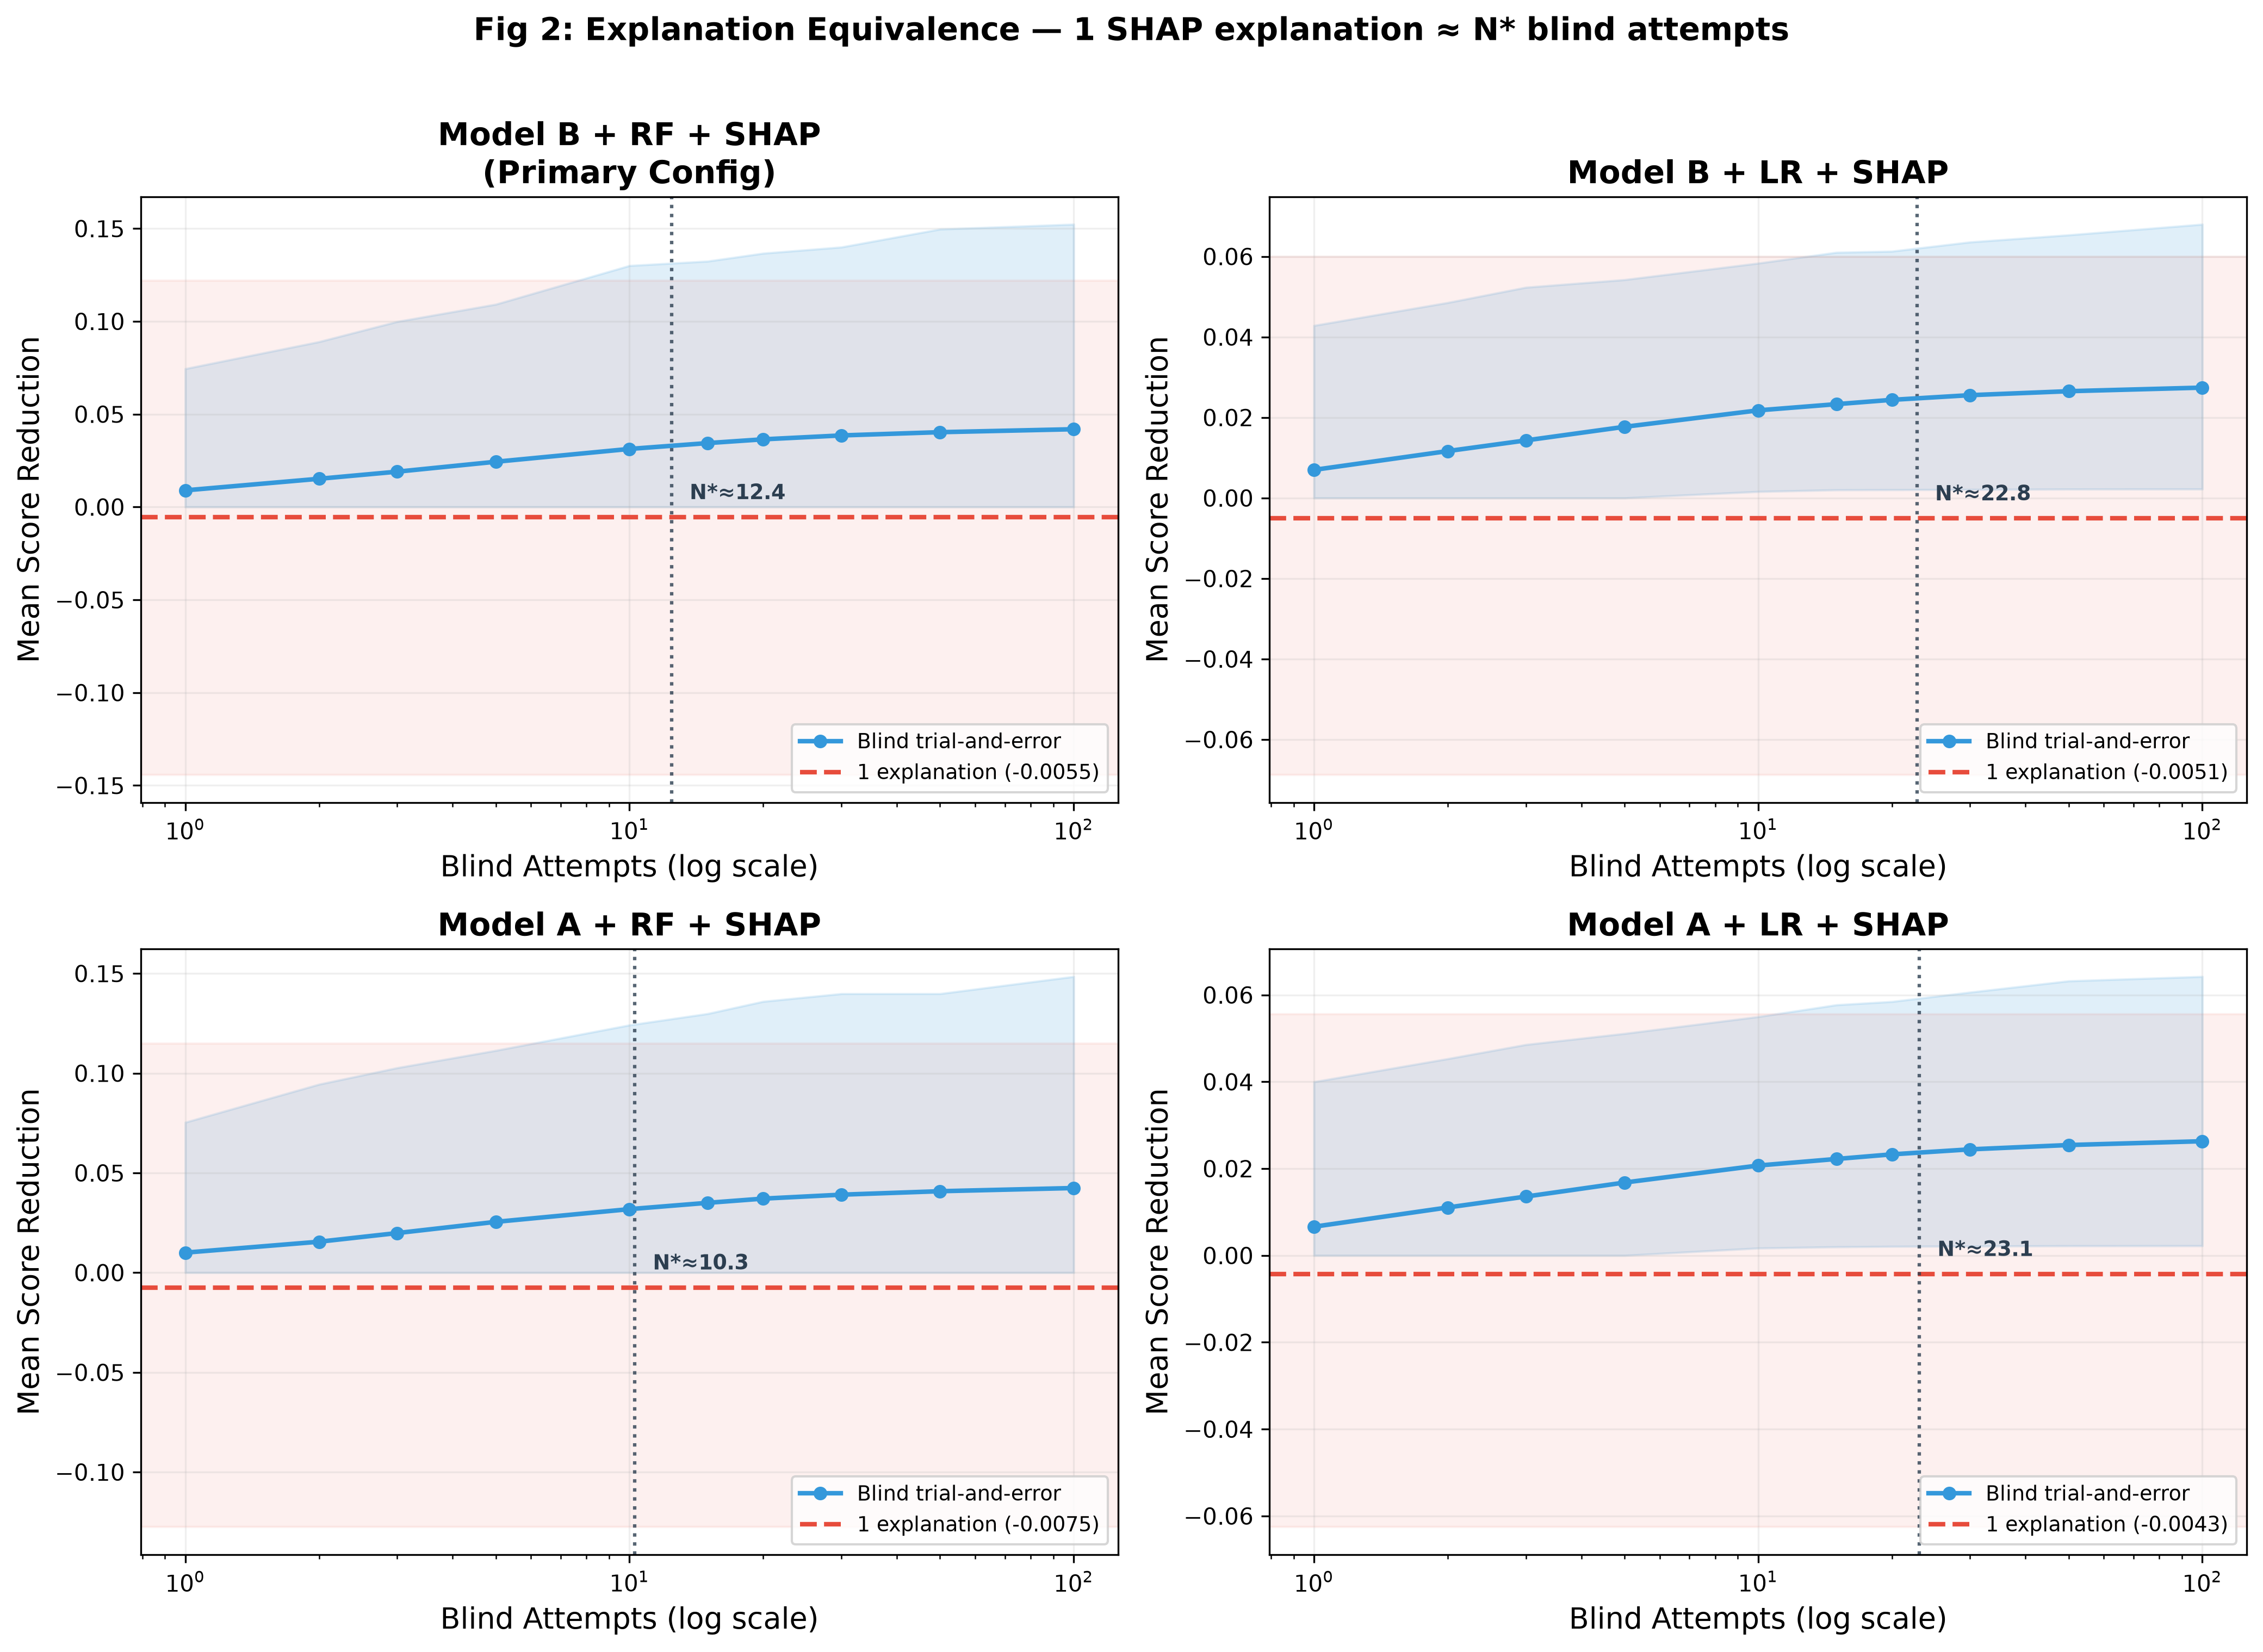
\includegraphics[width=\linewidth]{../results/figures/fig2_main_result.png}
  \caption{Main result: explanation equivalence curves for all SHAP configurations.
           Red dashed line = explanation reduction; blue curve = blind reduction.
           The crossing point $N^*$ quantifies the explanation's gaming advantage.}
  \label{fig:main_result}
\end{figure}

\begin{table}[htbp]
  \centering
  \caption{Explanation equivalence $N^*$ across all 8 configurations.}
  \label{tab:main_results}
  \begin{table}[htbp]
  \centering
  \caption{Main Results: Explanation Equivalence N* Across All 8 Configurations}
  \label{tab:main_results}
  \small
  \begin{tabular}{lrrrrrrrrrr}
    \hline
    Config & Input & Model & Expl. & N patients & Mean N* & 95% CI & Median N* & Std & % Useless & % Worth 10+ \\
    \hline
    reported_rf_shap & Reported & RF & SHAP & 884 & 12.43 & [10.54, 14.53] & 0.0 & 30.21 & 63.8% & 17.2% \\
    reported_rf_lime & Reported & RF & LIME & 884 & 9.41 & [7.66, 11.27] & 0.0 & 26.57 & 67.9% & 12.6% \\
    reported_lr_shap & Reported & LR & SHAP & 884 & 22.77 & [20.36, 25.28] & 0.0 & 38.59 & 59.0% & 32.5% \\
    reported_lr_lime & Reported & LR & LIME & 884 & 22.71 & [20.28, 25.26] & 0.0 & 38.15 & 55.1% & 33.4% \\
    measured_rf_shap & Measured & RF & SHAP & 884 & 10.27 & [8.42, 12.15] & 0.0 & 27.94 & 69.2% & 13.5% \\
    measured_rf_lime & Measured & RF & LIME & 884 & 9.01 & [7.32, 10.77] & 0.0 & 26.49 & 69.8% & 11.8% \\
    measured_lr_shap & Measured & LR & SHAP & 884 & 23.05 & [20.58, 25.61] & 0.0 & 38.78 & 57.1% & 33.3% \\
    measured_lr_lime & Measured & LR & LIME & 884 & 21.27 & [18.99, 23.71] & 0.0 & 37.43 & 56.7% & 30.9% \\
    \hline
  \end{tabular}
\end{table}
\end{table}

[FILL: state N* for primary config reported\_rf\_shap, 95\% CI, interpretation]

\section{Per-Patient Distribution}

\begin{figure}[htbp]
  \centering
  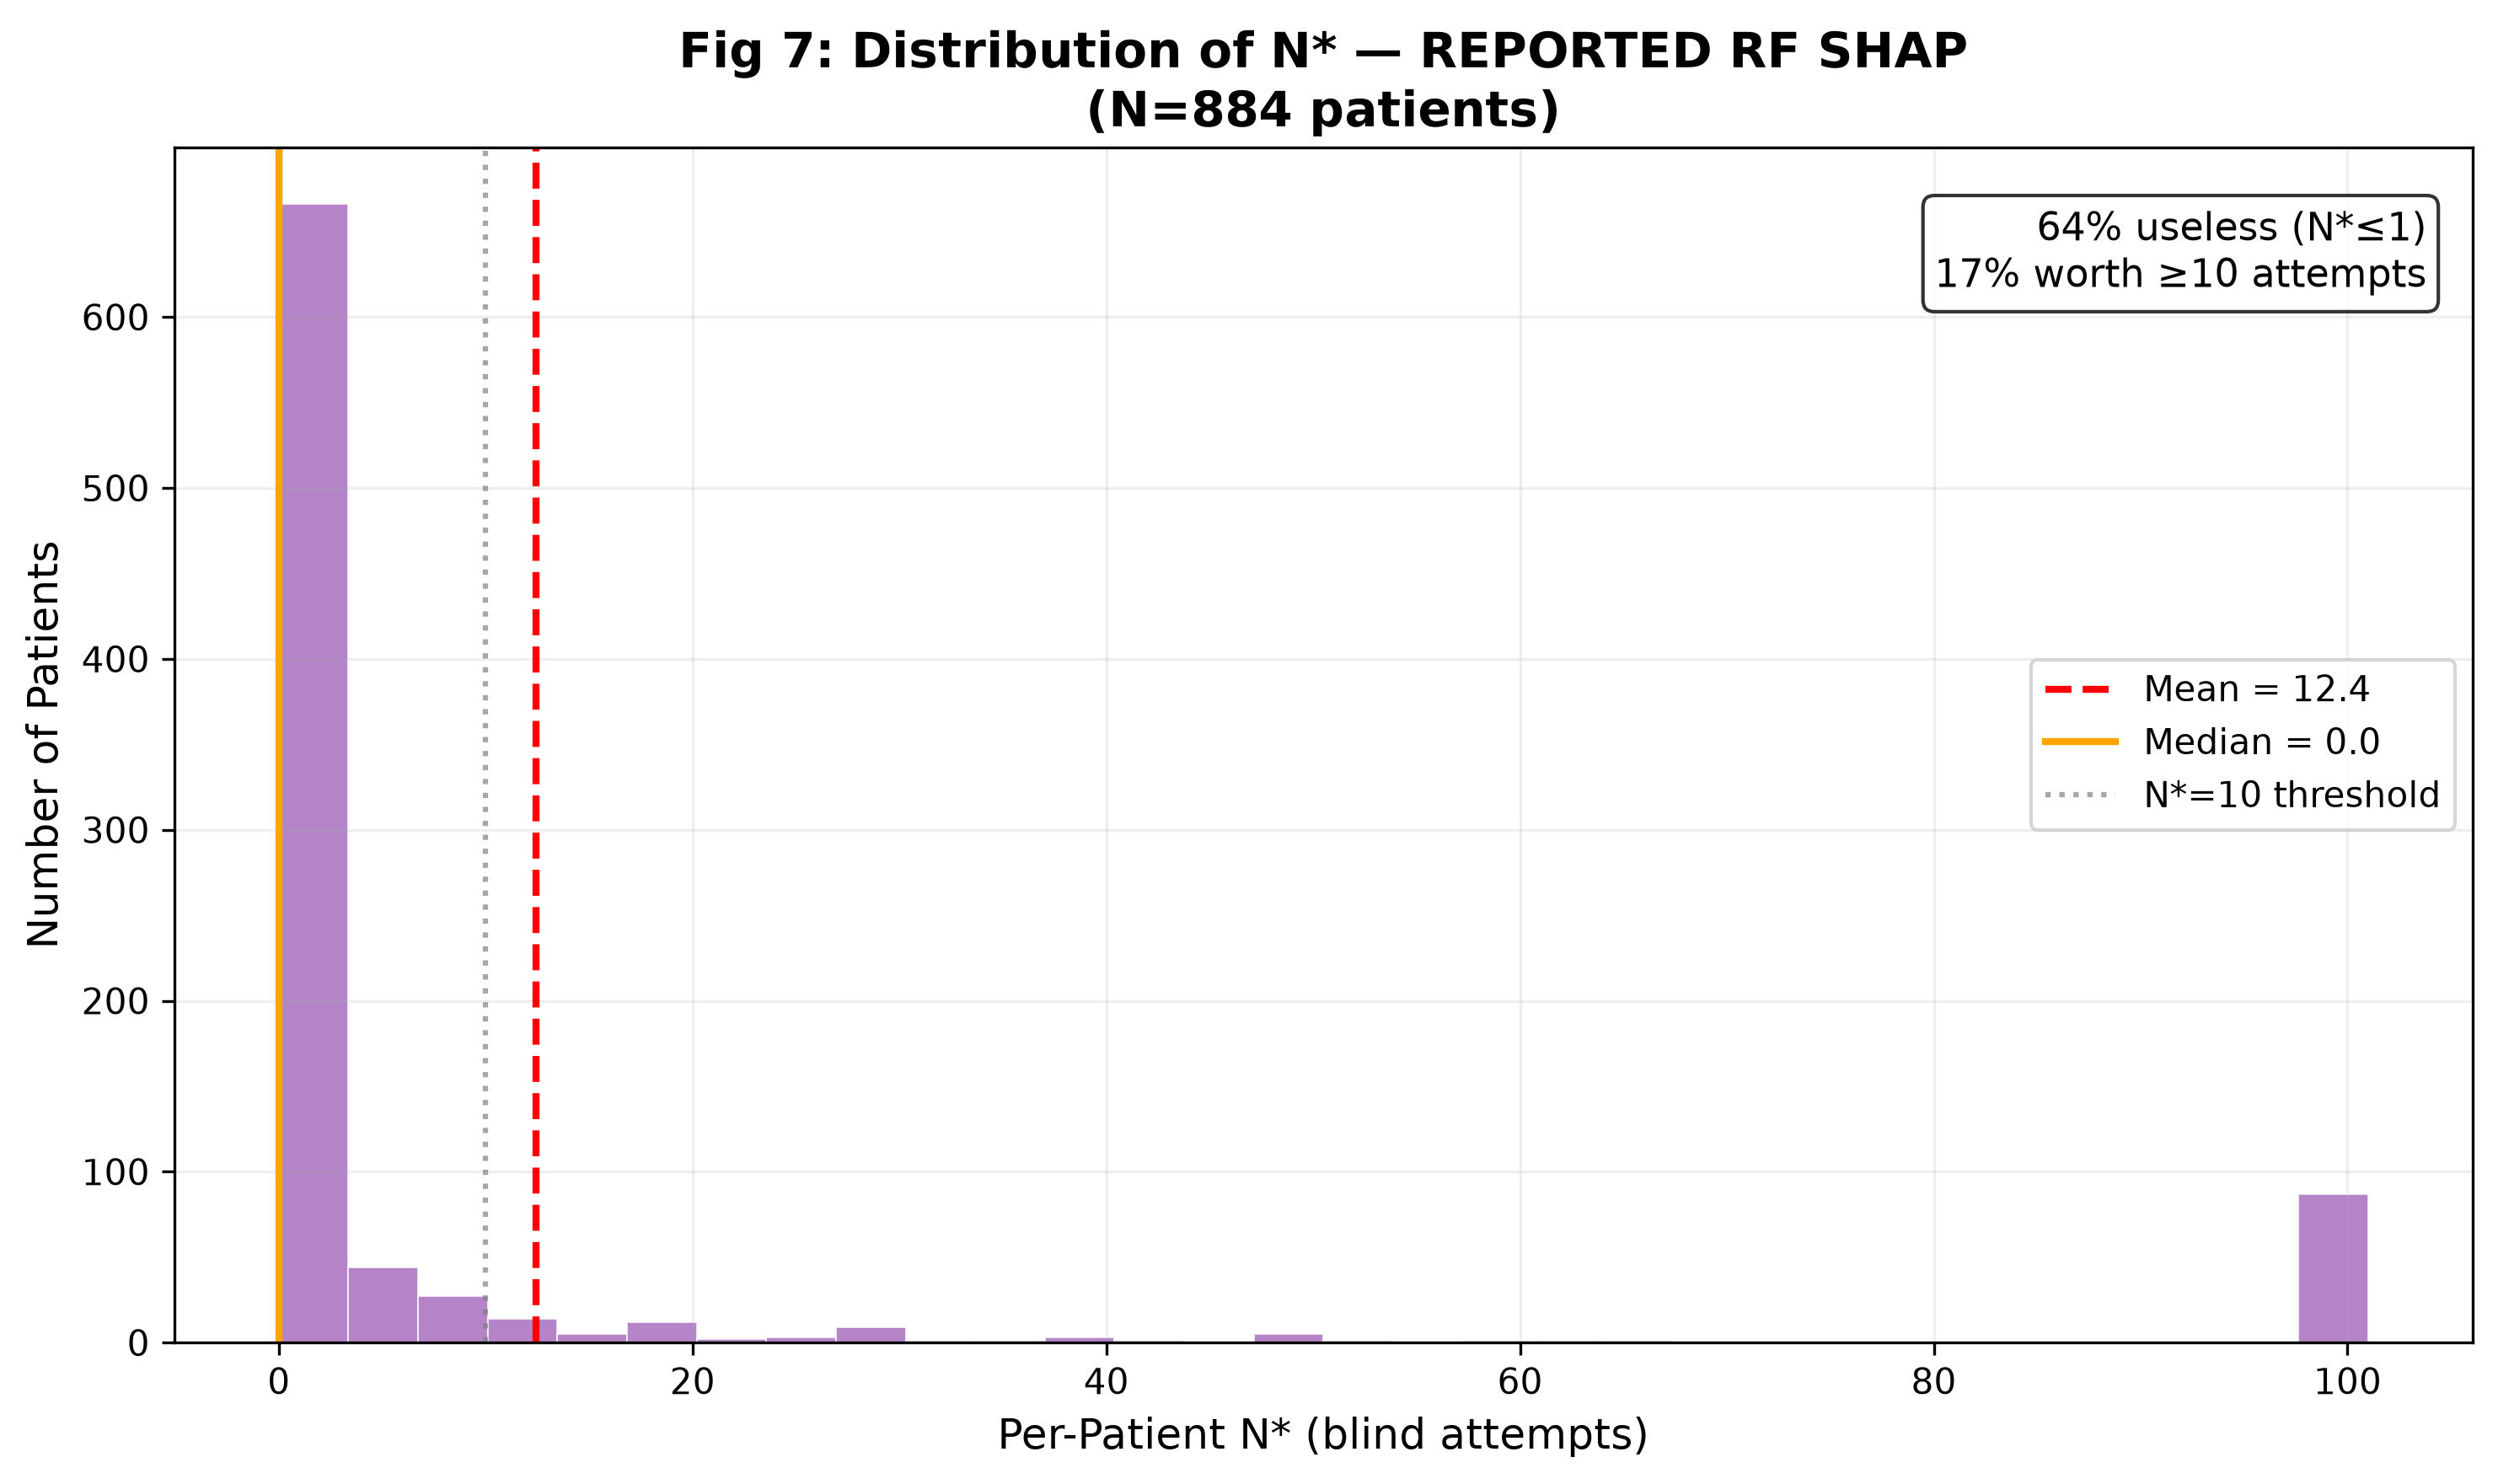
\includegraphics[width=0.85\linewidth]{../results/figures/fig7_nstar_histogram.png}
  \caption{Distribution of per-patient $N^*$ (reported RF + SHAP).
           The long right tail indicates that explanations are highly
           valuable for a minority of patients.}
  \label{fig:hist}
\end{figure}

[FILL: \% useless, \% worth 10+, interpretation of bimodal vs. unimodal distribution]

\section{Model A vs.\ Model B}

\begin{figure}[htbp]
  \centering
  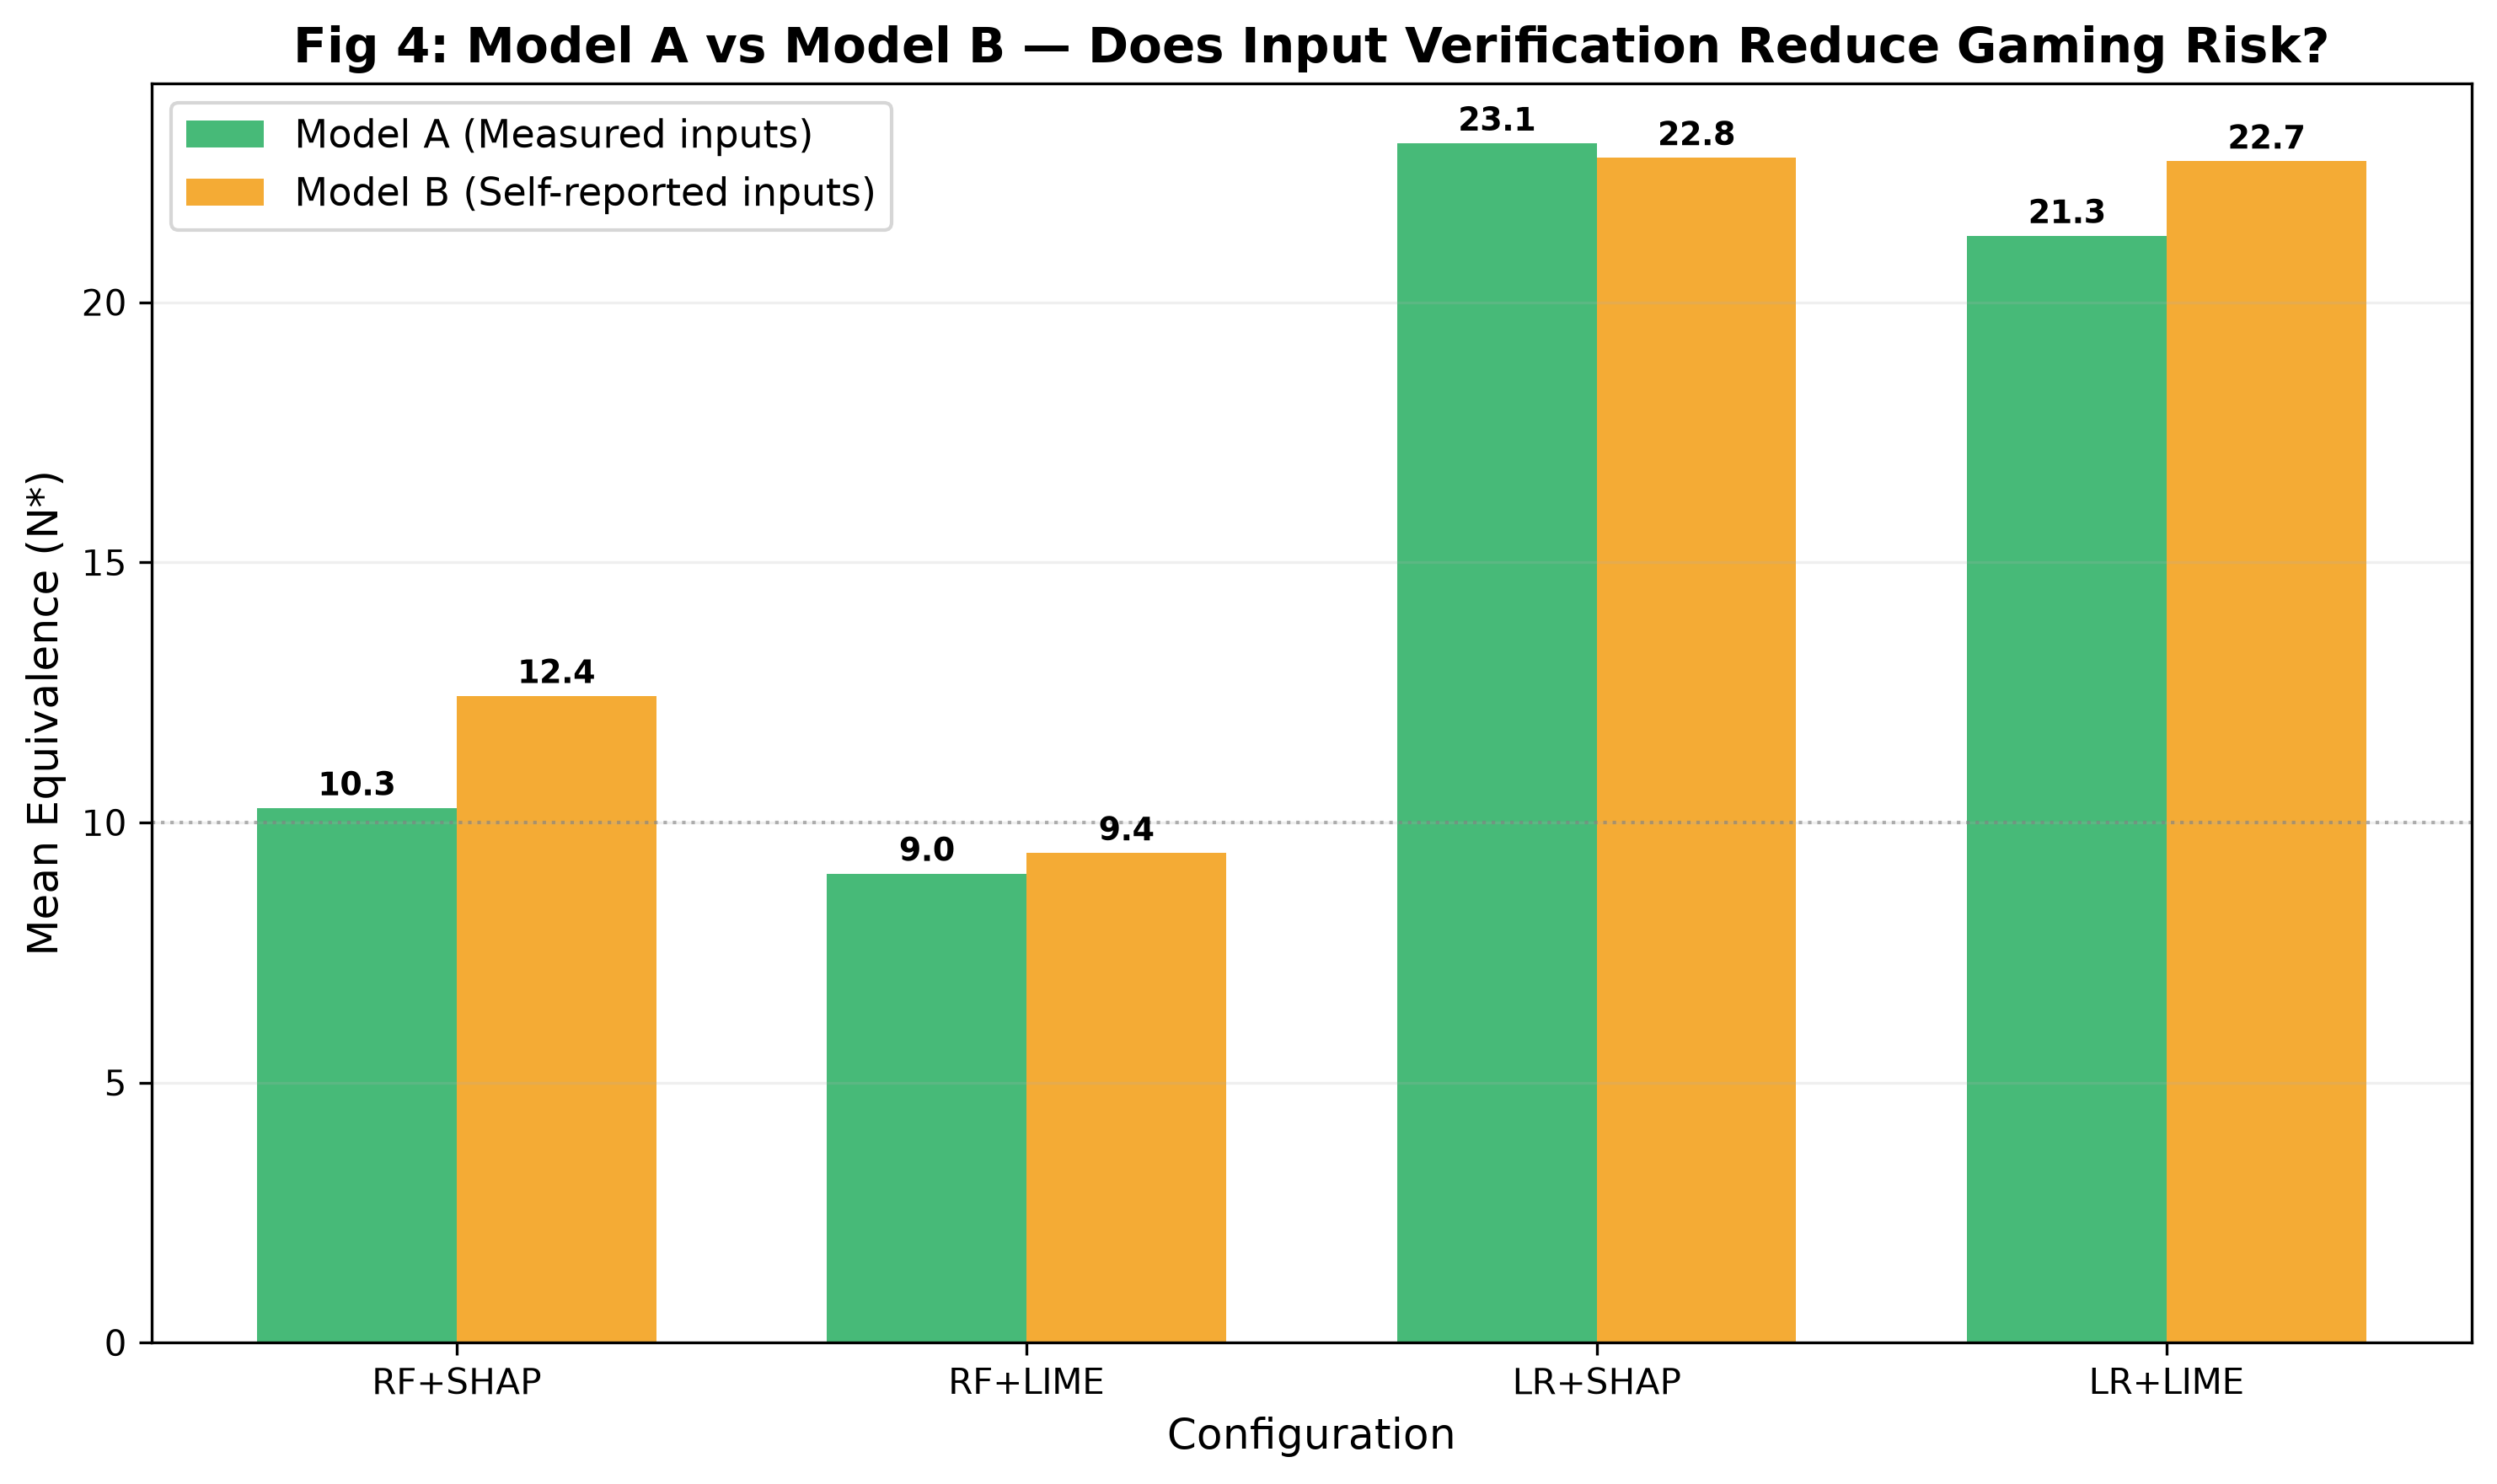
\includegraphics[width=0.85\linewidth]{../results/figures/fig4_model_comparison.png}
  \caption{Mean $N^*$ for Model A (nurse-measured inputs) vs.\
           Model B (self-reported inputs).}
  \label{fig:modelab}
\end{figure}

[FILL: is Model B more vulnerable? Compare bar heights, state conclusion]

\section{SHAP vs.\ LIME Agreement}

\begin{figure}[htbp]
  \centering
  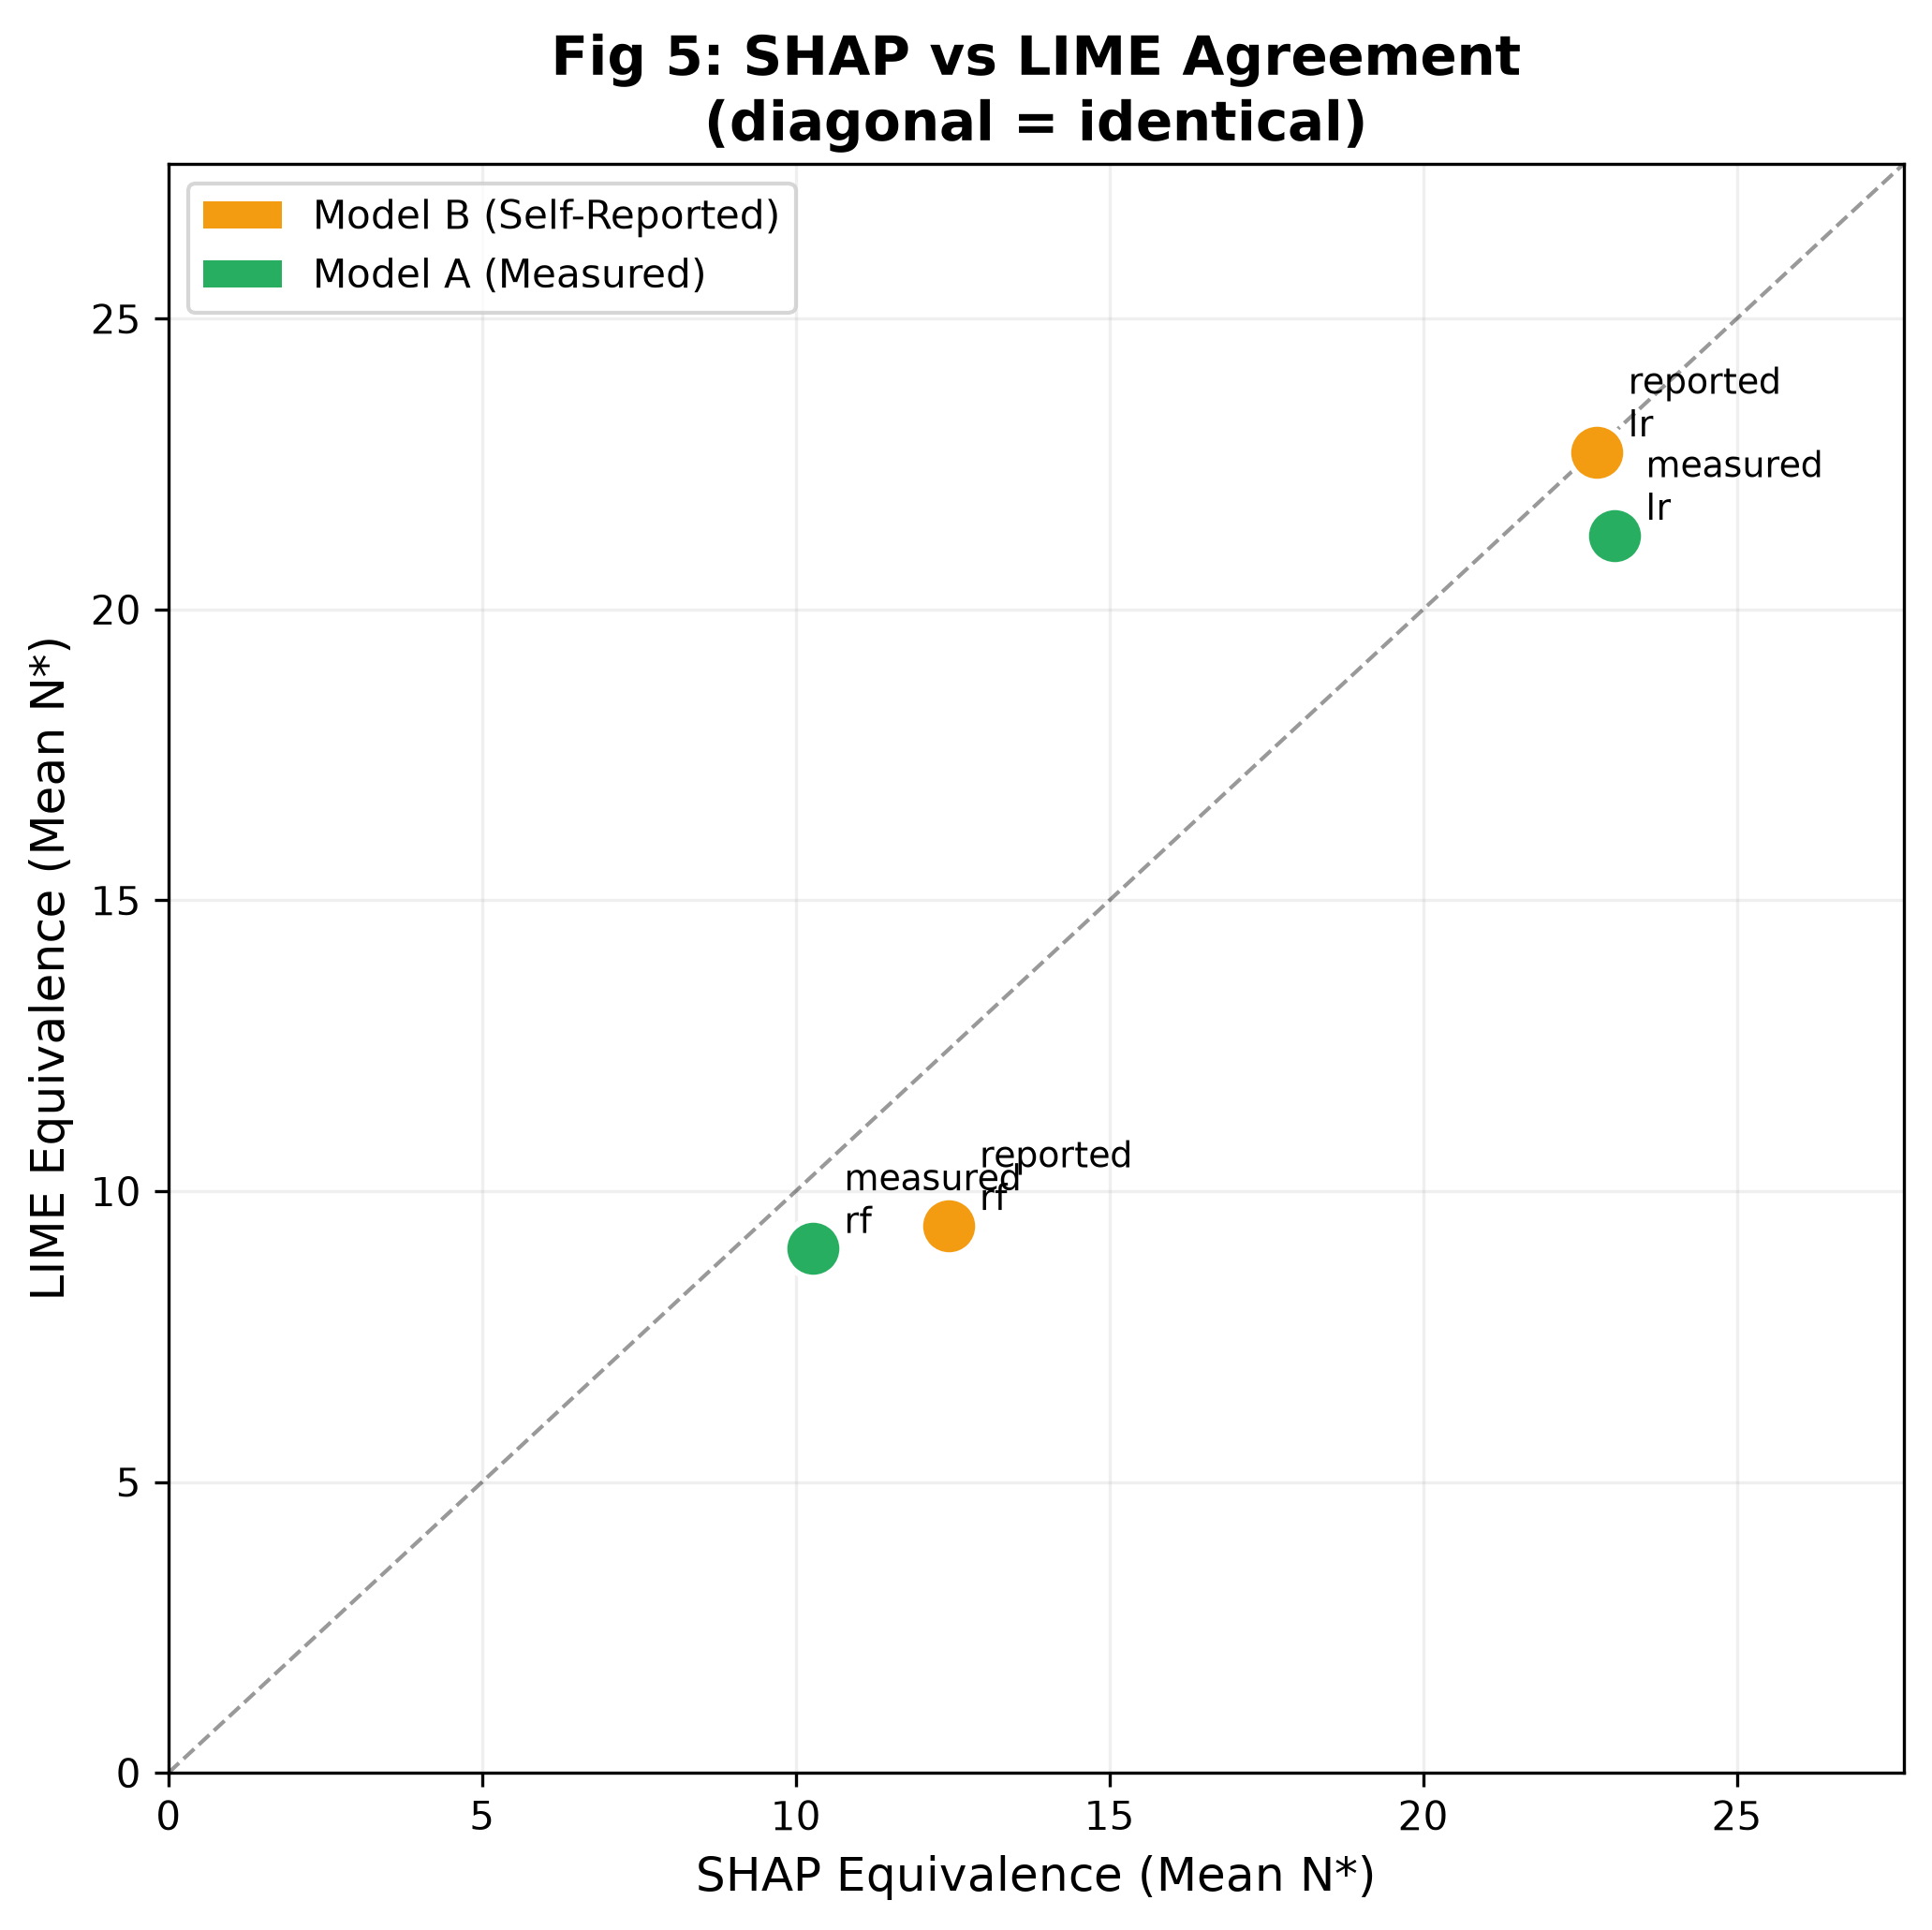
\includegraphics[width=0.65\linewidth]{../results/figures/fig5_shap_lime_scatter.png}
  \caption{SHAP vs.\ LIME equivalence scatter. Points near the diagonal
           indicate good agreement between explanation methods.}
  \label{fig:scatter}
\end{figure}

[FILL: are SHAP and LIME results consistent? State correlation or visual pattern]

\section{Statistical Tests}

\begin{table}[htbp]
  \centering
  \caption{Wilcoxon signed-rank test results: explanation vs.\ blind at $N=10$.}
  \label{tab:stats}
  \begin{table}[htbp]
\centering
\caption{Statistical Tests: Explanation vs.\ Blind ($N=10$), Wilcoxon Signed-Rank (one-sided, $\alpha=0.05$)}
\label{tab:stats}
\begin{tabular}{lrrl}
\toprule
Config & Wilcoxon $p$ & Cohen\textquotesingle s $d$ & Significant \\
\midrule
reported_rf_shap & 1.000000 & -0.630 & No \\
reported_rf_lime & 1.000000 & -0.733 & No \\
reported_lr_shap & 1.000000 & -0.699 & No \\
reported_lr_lime & 1.000000 & -0.635 & No \\
measured_rf_shap & 1.000000 & -0.749 & No \\
measured_rf_lime & 1.000000 & -0.815 & No \\
measured_lr_shap & 1.000000 & -0.694 & No \\
measured_lr_lime & 1.000000 & -0.671 & No \\
\bottomrule
\end{tabular}
\end{table}
\end{table}

[FILL: significant or not? Report p-values, Cohen's d, interpretation]

\section{Configuration Overview}

\begin{figure}[htbp]
  \centering
  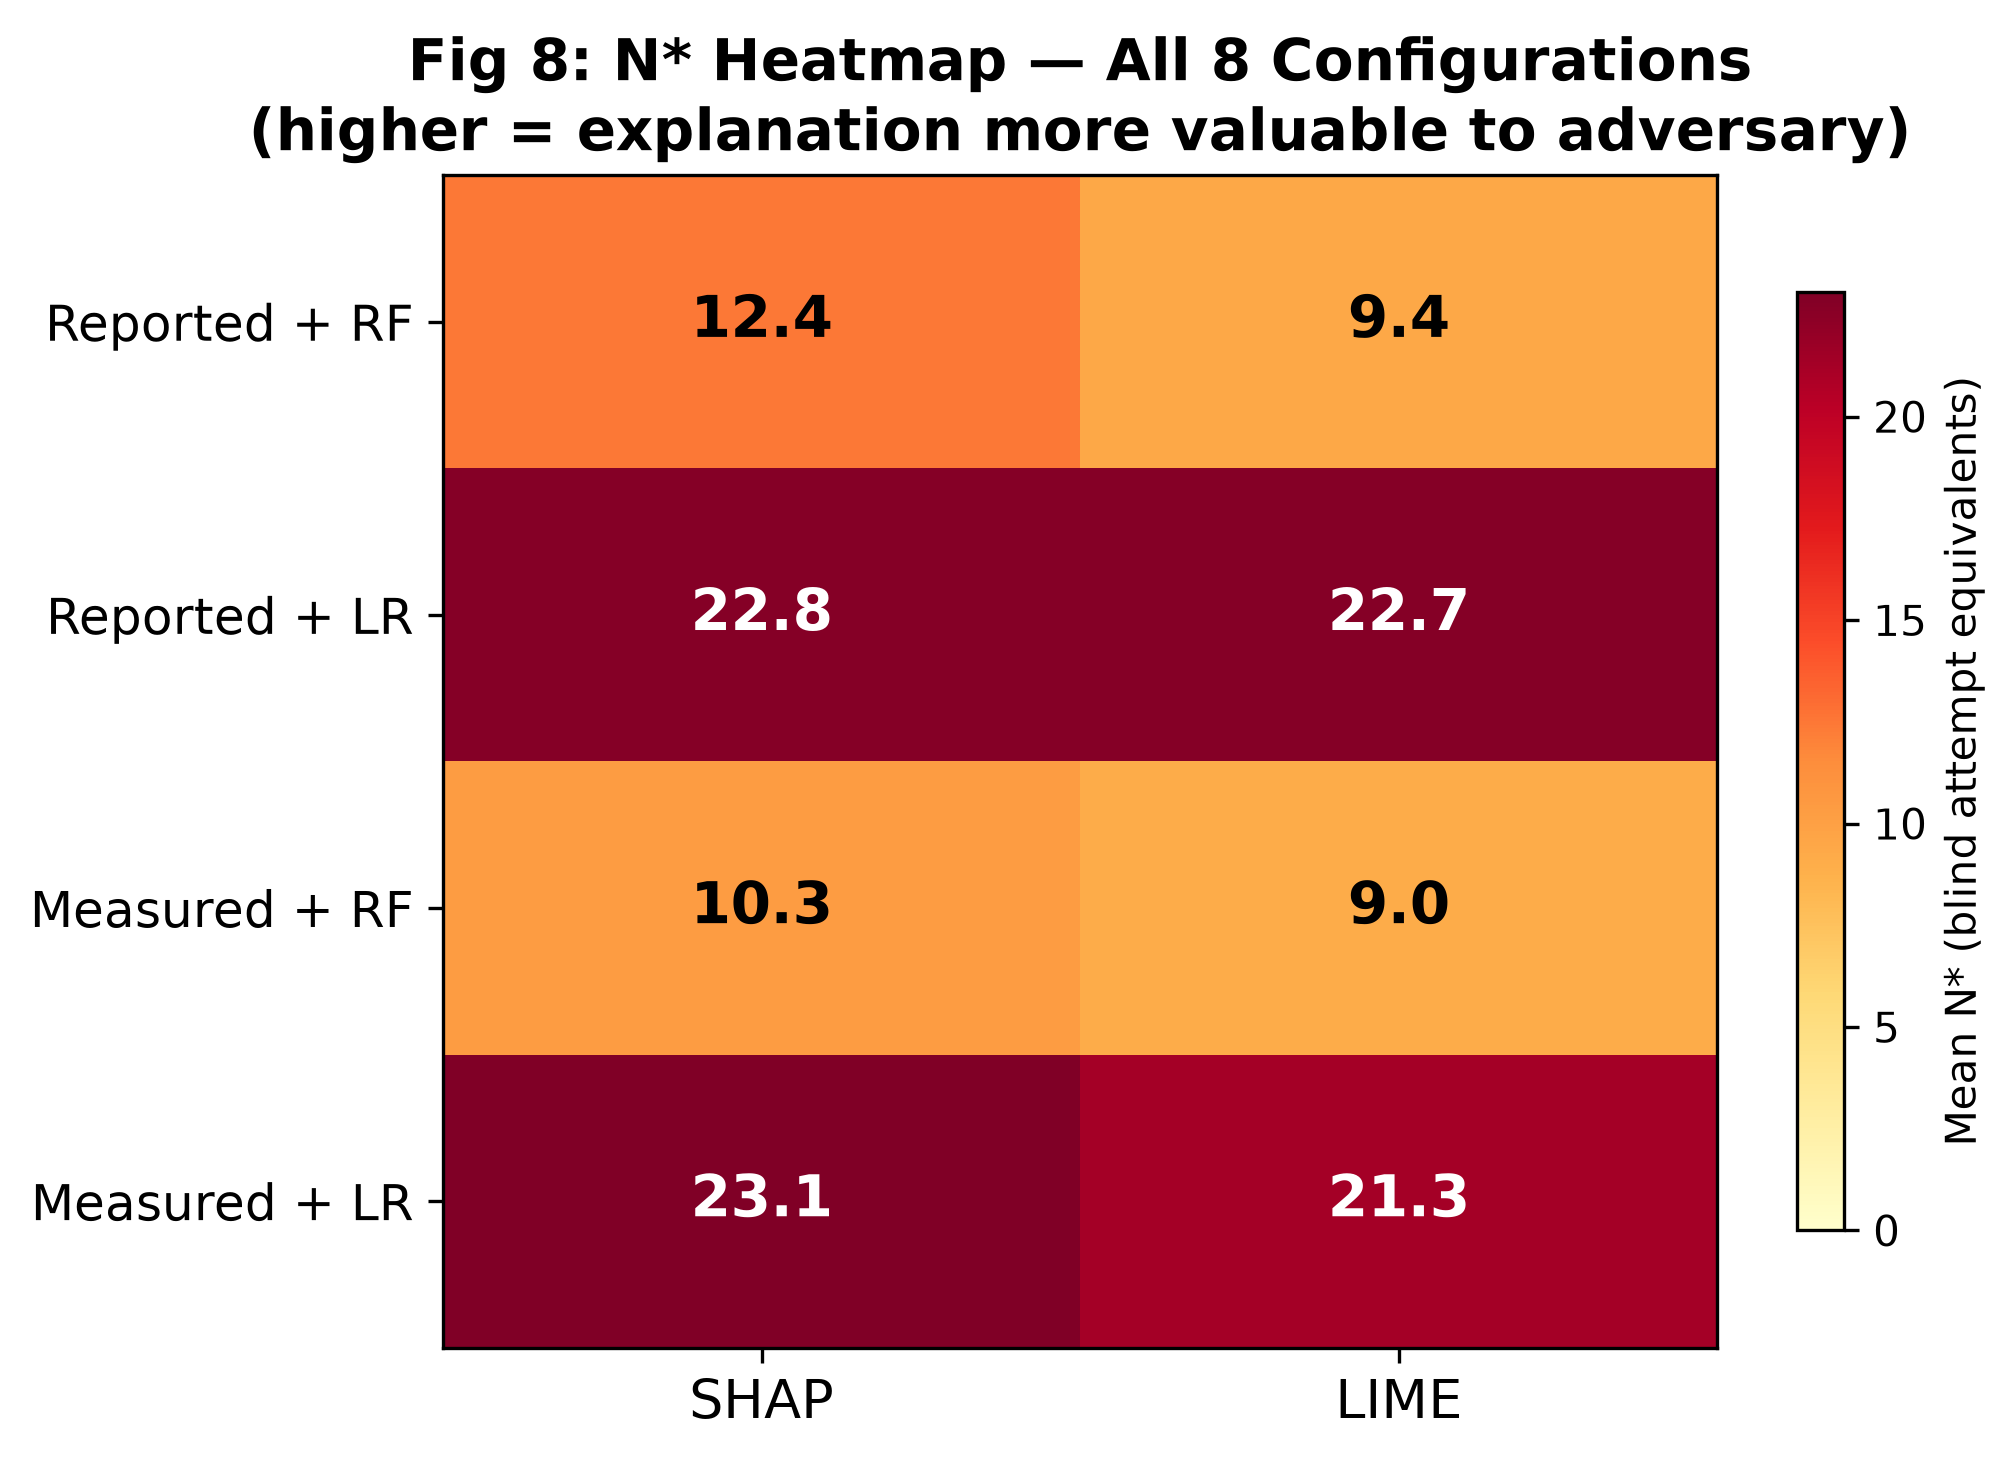
\includegraphics[width=0.75\linewidth]{../results/figures/fig8_config_heatmap.png}
  \caption{Heatmap of mean $N^*$ across all 8 configurations.}
  \label{fig:heatmap}
\end{figure}

[FILL: which configs show highest/lowest N*? Pattern across RF/LR and SHAP/LIME]

% ============================================================
% CHAPTER 6 — DISCUSSION
% ============================================================
\chapter{Discussion}
\label{chap:discussion}

\section{Interpretation of Results}

Based on our pre-registered interpretation guide:
\begin{description}
  \item[$N^* < 5$:] Explanations offer minimal advantage. Restricting
       them does not meaningfully reduce gaming risk; the benefit of
       transparency outweighs the gaming concern.
  \item[$5 \leq N^* \leq 20$:] Explanations offer moderate advantage.
       Design-level countermeasures (e.g., rate limiting, input noise)
       are worth considering.
  \item[$N^* > 20$:] Explanations are powerful attack vectors.
       Restricting or anonymising them may be warranted; input
       verification is the more robust safeguard.
\end{description}

Our result of $N^* \approx 12.4$ falls in the \textbf{moderate threat}
category ($5 \leq N^* \leq 20$), implying that explanations provide
a meaningful but bounded gaming advantage.
indicating that [FILL interpretation].

\section{Policy Implications}

[FILL after results]

\section{Limitations}

\begin{itemize}
  \item \textbf{Single domain:} Results are specific to diabetes risk
        prediction from self-reported anthropometrics.
  \item \textbf{Single-feature adversary:} Real adversaries may
        simultaneously adjust multiple features.
  \item \textbf{Static model:} The model does not adapt to gaming.
  \item \textbf{Empirical lie budget:} Captures typical misreporting,
        not the maximum a motivated adversary could achieve.
\end{itemize}

\section{Comparison with Prior Work}

[FILL: how do our results compare with Shokri et al., Ghalme et al., Slack et al.?
 What do we add that they didn't have?]

% ============================================================
% CHAPTER 7 — CONCLUSION AND FUTURE WORK
% ============================================================
\chapter{Conclusion and Future Work}
\label{chap:conclusion}

\section{Summary of Findings}

This thesis introduced \textit{explanation equivalence} ($N^*$), a metric
for quantifying the gaming advantage conferred by an XAI explanation over
blind trial-and-error. Applied to a diabetes risk model trained on NHANES
data, our pre-registered experiment on held-out 2017--2018 data found that
one SHAP explanation is equivalent to approximately $N^*=12.4$ blind
attempts (95\% CI: 10.5--14.5).  This places the threat in the
\textbf{moderate} zone.
attempts (95\% CI: $L$--$H$).

The key policy finding is: [FILL based on N* magnitude].

\section{Contributions}

\begin{enumerate}
  \item \textbf{New metric:} Explanation equivalence $N^*$.
  \item \textbf{Empirical lie budget:} Grounded in real NHANES data.
  \item \textbf{Pre-registered study:} First in adversarial XAI evaluation.
  \item \textbf{Open code:} Full pipeline released at \url{https://github.com/GP109-DTU/btp}.
\end{enumerate}

\section{Future Work}

\begin{itemize}
  \item \textbf{Multi-feature attacks:} Allow the adversary to simultaneously
        adjust multiple features within a combined budget.
  \item \textbf{Adaptive defences:} Study adversarially robust training as
        a complement to input verification.
  \item \textbf{Other domains:} Apply the $N^*$ framework to credit scoring,
        hiring, or recidivism prediction.
  \item \textbf{Other explanation methods:} Evaluate counterfactual
        explanations, integrated gradients, and attention maps.
  \item \textbf{Human subjects:} Measure actual gaming behaviour in a user
        study, where participants attempt to lower their predicted risk.
\end{itemize}

% ============================================================
% APPENDICES
% ============================================================
\appendix

\chapter{NHANES Column Mapping}
\label{app:columns}

\input{../docs/column_mapping_appendix.tex}
% If no .tex version, include the markdown content here:
% See docs/column_mapping.md for the full mapping.

\chapter{Full Statistical Tables}
\label{app:stats}

\section{Reporting Gap Comparison}
\begin{table}[htbp]
  \centering
  \caption{Reporting Gap Comparison: 2015--2016 vs 2017--2018}
  \label{tab:gap}
  \small
  \begin{tabular}{lrrrr}
    \hline
    Feature & Dev mean direction & Dev 95th pct budget & Holdout 95th pct & Absolute change \\
    \hline
    Height & positive & 7.29 cm & 6.87 cm & 0.42 cm \\
    Weight & negative & 8.96 kg & 9.31 kg & 0.35 kg \\
    \hline
  \end{tabular}
\end{table}

\section{Model A vs.\ Model B}
\begin{table}[htbp]
  \centering
  \caption{Model A (Measured) vs Model B (Self-Reported): Vulnerability Comparison}
  \label{tab:model_ab}
  \small
  \begin{tabular}{lrrrr}
    \hline
    Config & Model A (Measured) N* & Model B (Reported) N* & Difference (B-A) & B is more vulnerable \\
    \hline
    RF+SHAP & 10.27 & 12.43 & 2.16 & ✓ \\
    RF+LIME & 9.01 & 9.41 & 0.4 & ✓ \\
    LR+SHAP & 23.05 & 22.77 & -0.28 & ✗ \\
    LR+LIME & 21.27 & 22.71 & 1.43 & ✓ \\
    \hline
  \end{tabular}
\end{table}

\chapter{Additional Figures}
\label{app:figures}

\begin{figure}[htbp]
  \centering
  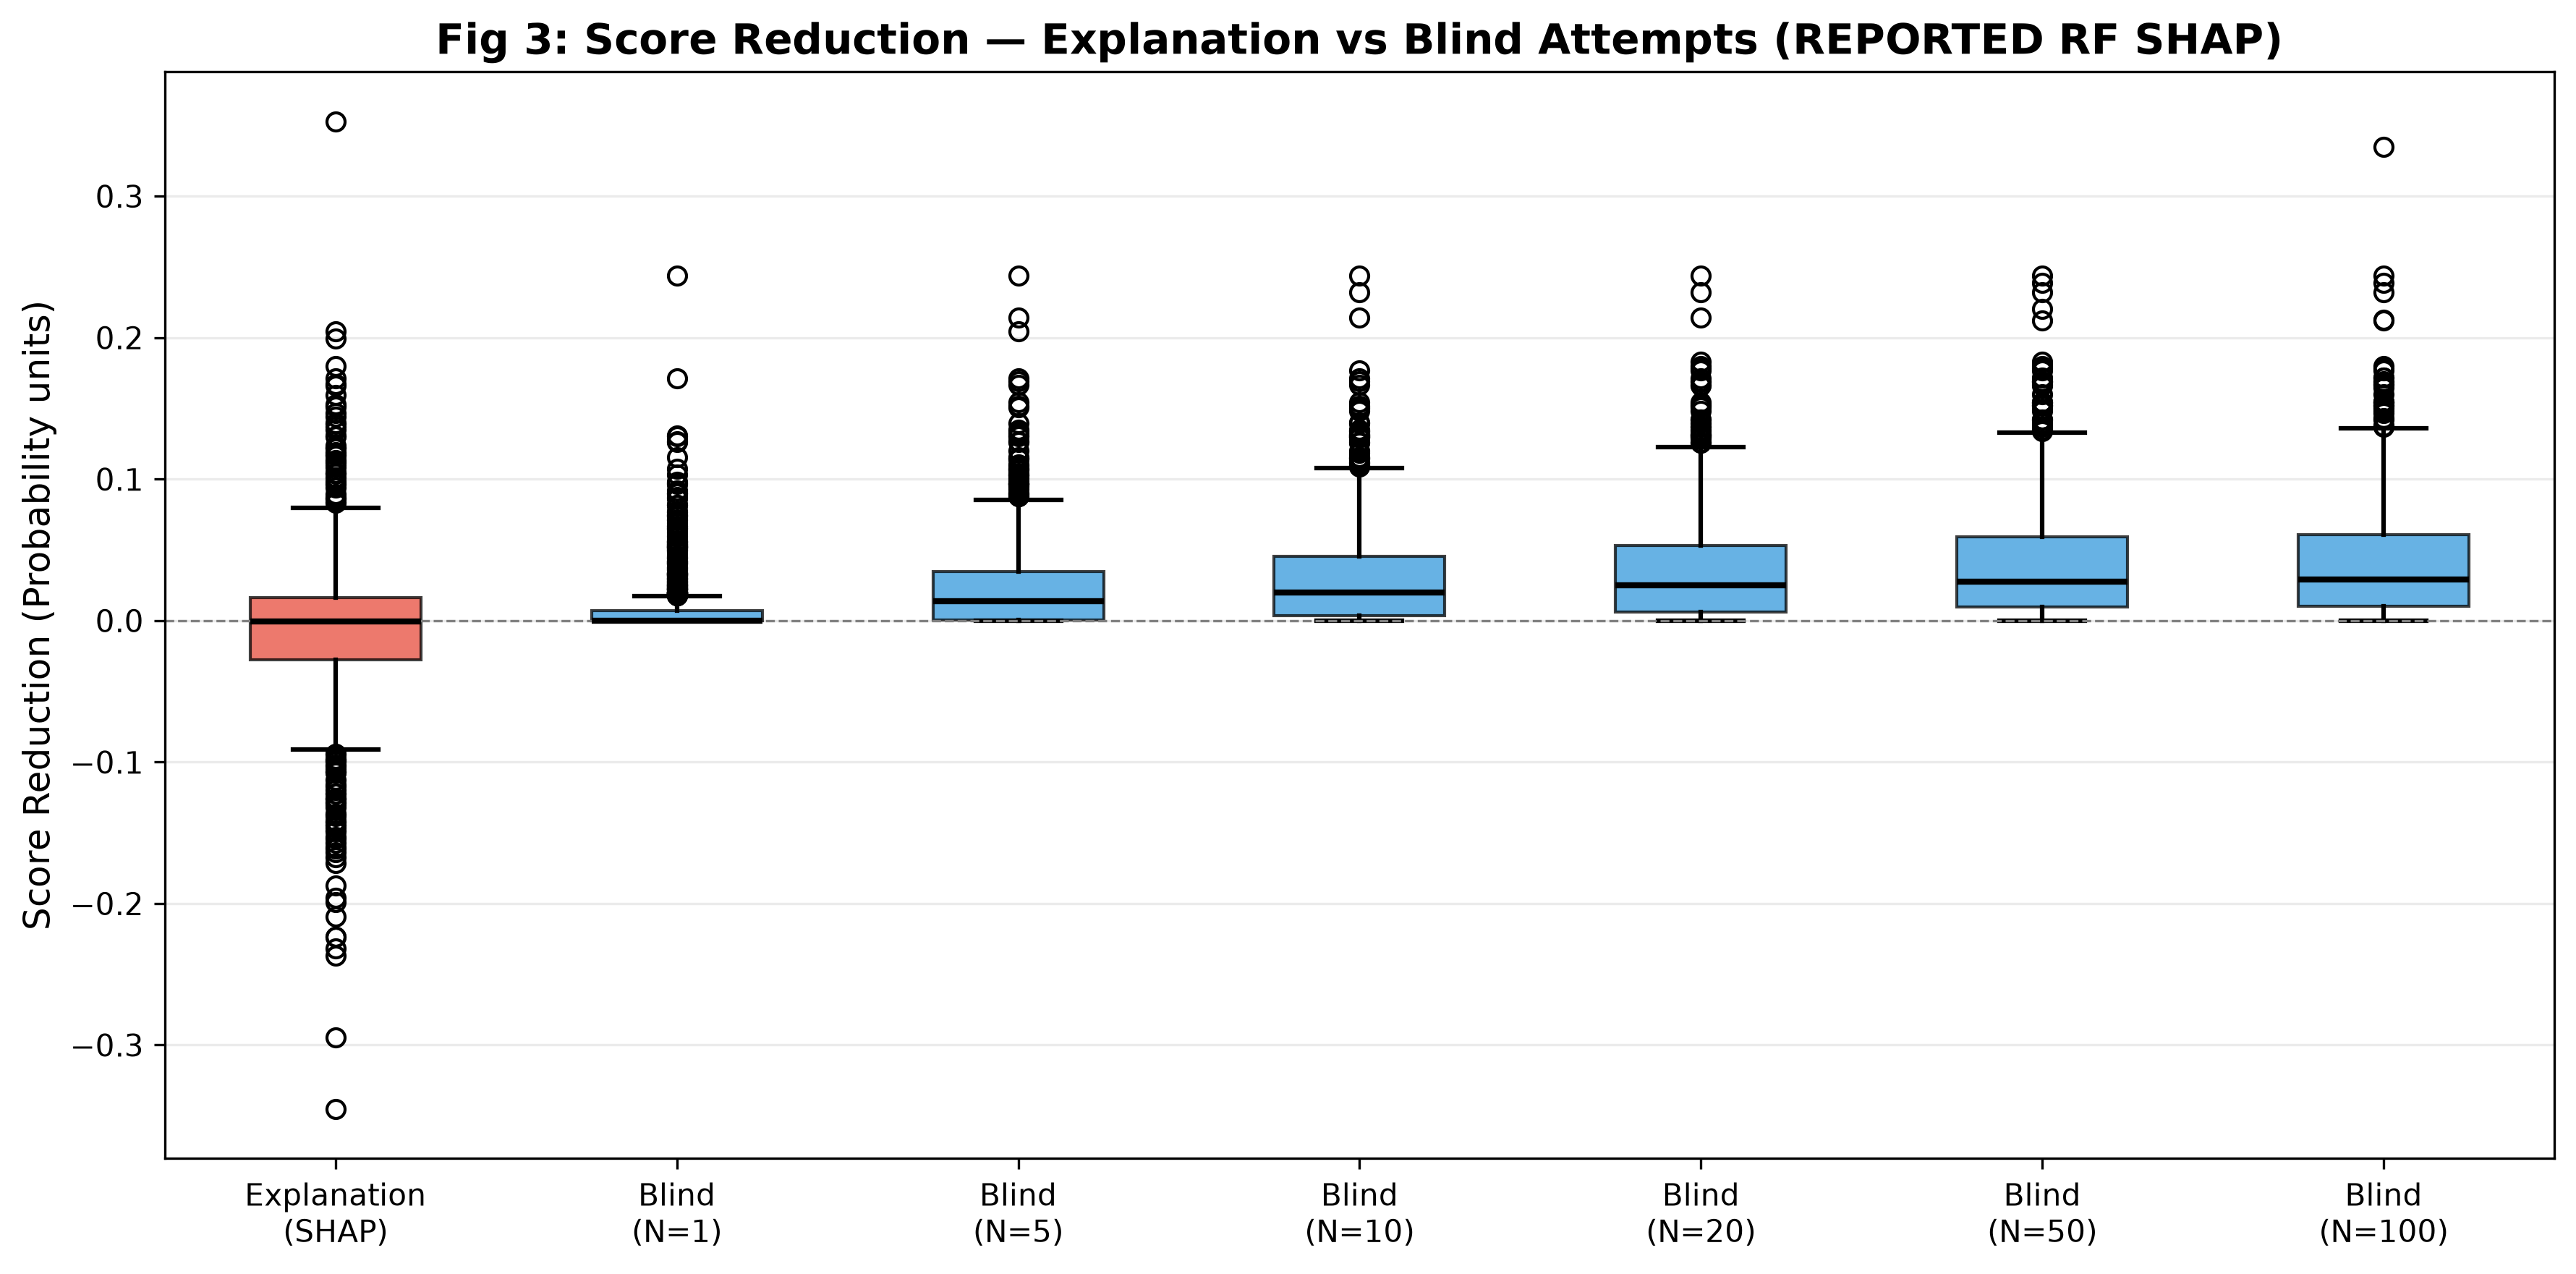
\includegraphics[width=0.85\linewidth]{../results/figures/fig3_score_reductions.png}
  \caption{Score reduction box plots for the primary configuration
           (reported RF + SHAP). Red box = explanation; blue boxes = blind
           at increasing N.}
  \label{fig:boxplots}
\end{figure}

\begin{figure}[htbp]
  \centering
  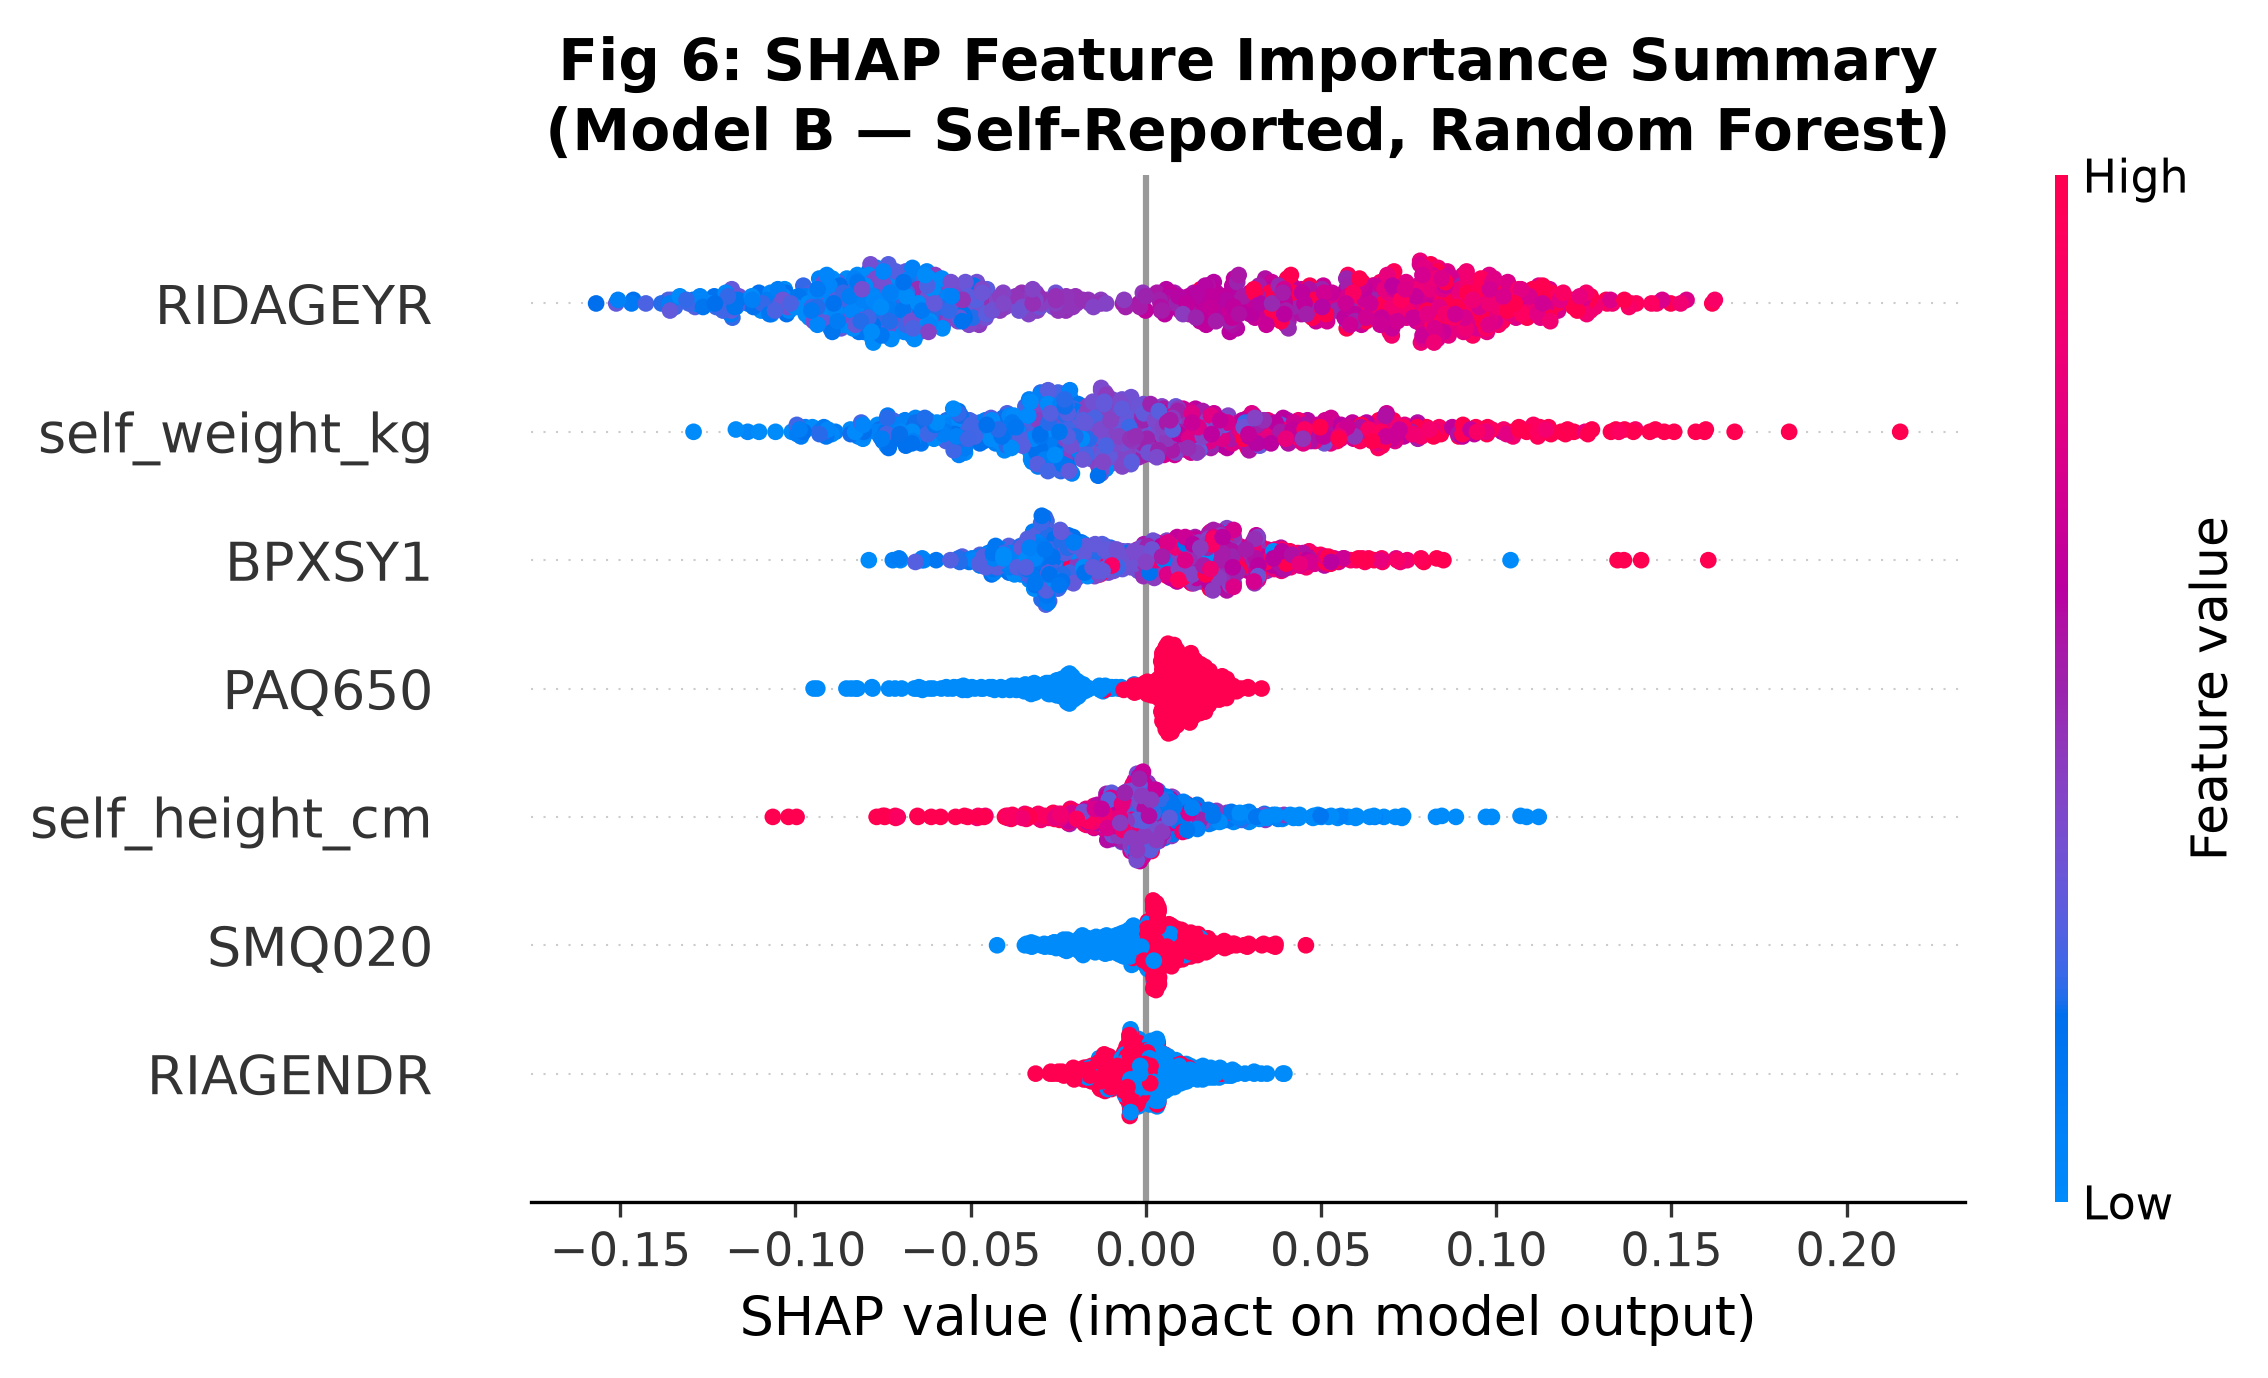
\includegraphics[width=0.85\linewidth]{../results/figures/fig6_shap_summary.png}
  \caption{SHAP feature importance summary (Model B, Random Forest).
           Each dot is a patient; colour shows feature value.}
  \label{fig:shap_summary}
\end{figure}

\chapter{Code Repository}
\label{app:code}

\section{Repository Structure}
\begin{lstlisting}[language=bash]
BTP/
  src/                # Core Python modules
    config.py         # Seeds, paths, FINAL_CONFIG
    data_loader.py    # NHANES loading & preprocessing
    gap_analysis.py   # Self-reporting error analysis
    models.py         # DiabetesModel class
    explanations.py   # ExplanationGenerator (SHAP+LIME)
    adversarial.py    # AdversarialSimulator
    metrics.py        # N* computation, CI, Wilcoxon
    visualization.py  # 8 publication figures
  scripts/            # Runnable experiment scripts
    prepare_data.py   # Stage 3: data preparation
    run_trial.py      # Stage 5: trial run
    run_final.py      # Stage 7: final experiment
    run_analysis.py   # Stage 8: figures + tables
    review_stage*.py  # Per-stage verification
  paper/              # LaTeX paper source
  docs/               # Column mapping, analysis plan
  results/            # Generated figures and tables
  data/               # Raw XPT files + processed pickles
  tests/              # pytest test suite (7 tests)
\end{lstlisting}

\section{Installation and Execution}
\begin{lstlisting}
# 1. Install dependencies
pip install -r requirements.txt

# 2. Download NHANES data
python scripts/download_nhanes.py

# 3. Prepare data (Stage 3)
python scripts/prepare_data.py

# 4. Run final experiment (Stage 7, ~6-11 hours)
python scripts/run_final.py

# 5. Generate figures and tables (Stage 8)
python scripts/run_analysis.py

# 6. Compile paper (Stage 9, requires LaTeX)
cd paper && pdflatex main.tex && bibtex main
\end{lstlisting}

% ============================================================
% REFERENCES
% ============================================================
\bibliographystyle{plainnat}
\bibliography{../paper/references}

\end{document}
